\documentclass{article}
\usepackage{geometry}
\geometry{a4paper,top=2cm,bottom=2cm,left=1.5cm,right=1.5cm,%
	heightrounded,bindingoffset=5mm} %sistemiamo questi per decidere i bordi
\usepackage[utf8]{inputenc}
\usepackage{wrapfig}
\usepackage{float}
\usepackage{caption}
\usepackage[cc]{titlepic}
\usepackage{graphicx}
\usepackage{natbib}
\usepackage{makecell}
\usepackage{graphicx}
\usepackage{multirow}
\usepackage[table,xcdraw]{xcolor}
\usepackage{color, colortbl}
\definecolor{Gray}{gray}{0.9}
\definecolor{LightCyan}{rgb}{0.88,1,1}
\usepackage[first=0,last=9]{lcg}
\newcommand{\ra}{\rand0.\arabic{rand}}

\newcommand{\specialcell}[2][c]{%
	\begin{tabular}[#1]{@{}c@{}}#2\end{tabular}}


\begin{document}
	
	\begin{titlepage}
		\centering
		
\includegraphics[width=0.80\textwidth]{marchio.jpg}\par\vspace{2cm}
		{\scshape\LARGE Data Mining Report \par}
		\vspace{1cm}
		{\scshape\Large Group 12 \\ \par}
		\vspace{1cm}
		{\huge\bfseries Analysis of car auctions\par}
		\vspace{2cm}
		{\Large\ Lorenzo Bellomo \\ Andrea Bruno \\ Marta Scalisi \\ Chiara Spampinato\par}
		\vspace{4cm}
		{\Large\ January 2020\par}
	\end{titlepage}
	
	
	
	
	\section{Data Understanding}
	The dataset contains information about car auctions occurred in the US between 2009 and 2010 by the company Carvana. In this section, we'll explain how we analysed the data and how we assessed the quality of them. Furthermore, we'll show how we fixed the problem of the missing values (both invalid and misleading).
	
	\subsection{Data Semantics}
	\label{sec:dataSemantics}
	The semantic meaning of the most important (in our opinion) variables in the dataset are described as follows. The remaining columns are not discussed either because their meaning is too obvious or because its discussion is delayed to the following sections.
	
	\begin{itemize}
		\item \emph{RefId}: a unique number ID assigned to each vehicle;
		\item \emph{Auction}: a categorical attribute which defines three different auction providers (Manheim, Adesa, other);
		\item \emph{Make}: a categorical attribute specifying the name of the company producing that vehicle;
		\item \emph{VehOdo}: a numerical discrete attribute that points out the mileage;
		\item \emph{VehBCost}: a continuous numerical attribute indicating the actual final auction price;
		\item \emph{MMRA}: four numerical attributes that define the acquisition price of each vehicle:
		\begin{enumerate}
			\item price for this vehicle in average condition at the time of purchase; 
			\item price for this vehicle in the above Average condition at the time of purchase;
			\item price for this vehicle in the retail market in average condition at the time of purchase;
			\item price for this vehicle in the retail market in above average condition at the time of purchase;
		\end{enumerate}
		\item \emph{MMRC}: four numerical attributes that define the current price of each vehicle:
		\begin{enumerate}
			\item price for this vehicle in average condition as of the current day;
			\item price for this vehicle in the above condition as of the current day;
			\item price for this vehicle in the retail market in average condition as of the current day;
			\item price for this vehicle in the retail market in above average condition as of the current day;
		\end{enumerate}
		\item \emph{IsBadBuy}: the target variable. It states if the car was a good deal or not;
	\end{itemize}
	
	Finally, by analyzing all the attributes, we noticed that \emph{Acquisition Type} and \emph{Kickdate} are not present in the dataset, although they are declared in the dictionary.
	
	\subsection{Variables transformation and elimination of redundant variables}
	We opted to specialize the attributes \emph{Model} and \emph{SubModel} because they contained too much information. As an example, we found a row having the \emph{Model} attribute set as follows: EQUINOX FWD V6 3.4L. 
	
	It's quite clear that the dataset needs a reorganization because, as it is, it does not even respect the first normal form. Hence, we reorganised this information into five different attributes as explained hereafter:
	\begin{itemize}
		\item \emph{EngineLiters}: this information was both in \emph{Model} and \emph{SubModel} column, usually in the form of a float number and an L character (i.e. 2.7L);
		\item \emph{NumCylinders}: this information was taken from both variables (i.e. V4, V-8, I4\dots);
		\item \emph{WheelDrive}: wheel drive configuration (i.e. 2WD, 4WD\dots);
		\item \emph{4X4}: four-wheel-drive derived from \emph{WheelDrive} (4X4 means 4WD);
		\item \emph{NumDoors}: the number of the doors in a car (i.e. 5D), extracted by \emph{SubModel};
	\end{itemize}
	
	The information contained in these new attributes is not very interesting in itself, but thanks to this approach, we were able to ”clean” both columns from their meta-information. As an example, the Model column passed from about 1000 unique models to just around 200 models without any loss of information. 
	
	Afterwards, we also created four different attributes to separate the information contained in the variable \emph{PurchDate}. In detail, we created: \emph{PurchYear, PurchMonth, PurchDay} and \emph{PurchWeekDay} (which is the working day of acquisition, like Monday, Tuesday\dots).
	
	For the sake of simplicity, from now on, the 8 MMR variables will be addressed with an abbreviation. For example, \emph{MMRAcquisitionRetailAveragePrice} becomes \emph{ARAP}, \emph{MMRCurrentAuctionCleanPrice} becomes \emph{CACP}, and so on.
	
	
	\begin{figure}[H]
		\centering
		{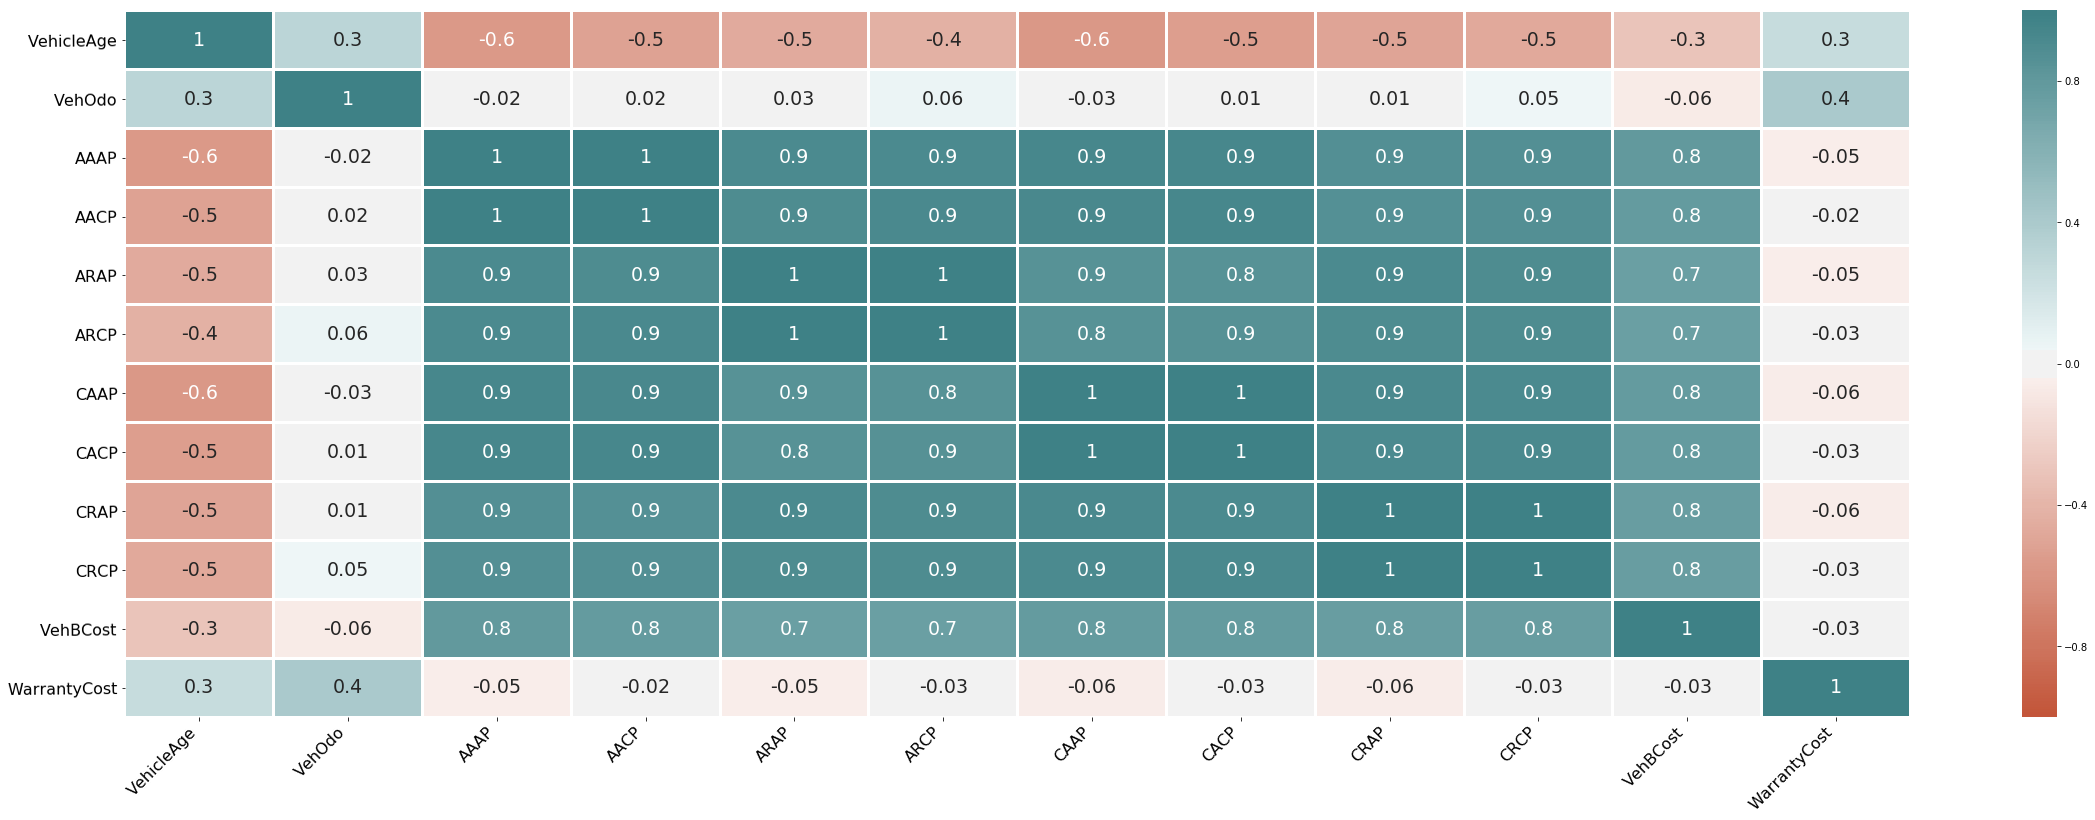
\includegraphics[width=\textwidth]{corr.png}}
		\caption{{ Correlation matrix }}
		\label{fig:corr}
	\end{figure}
	
	The correlation matrix in Figure \ref{fig:corr} reveals that all the \emph{MMRs} are strongly correlated (close to 0.9). Consequently, we chose to squeeze them using the PCA technique into two attributes called \emph{PCA1} and \emph{PCA2}. The first one became the most correlated to the original prices, whereas the second one was principally expressing the variance between the observations. For the sake of clarity, we used \emph{PCA1} and \emph{PCA2} only in Section \ref{sec:classification}, while dealing with classification.
	
	Do note that during the pattern mining and the clustering phases, we reintroduced \emph{MMRAcquisitionAuctionAveragePrice} (or \emph{AAAP}), because we needed to have clearer semantics regarding car prices. \\
	The discussion regarding the distribution of \emph{MMR} attributes and \emph{PCA} is delayed to Section \ref{sec:attrDistr}.
	
	\subsection{Assessing data quality}
	
	To assess the quality of the data, we performed some variable wise consistency checks (for example on \emph{VehYear, VehicleAge, VehOdo, WarrantyCost}), but we did not find any notable error.
	We noticed in the dataset some values with inconsistent naming (for example a pair of Japanese cars labelled as American or one model named in two different ways), and we manually fixed those errors.
	Nevertheless, we found a lot of 0 values for the 8 \emph{MMR} prices (in addition to their missing values), and we also identified one clear outlier in the \emph{VehBCost} column, with this car having been sold at 10\$. We then decided to drop this row.
	
	As far as the outliers are concerned, we found that the \emph{MMR} prices were usually coherent with respect to the \emph{VehBCost} attribute, so we decided to keep in the data set all the other rows. In this, we also kept a lot of very expensive cars, but we could not label these cars as outliers, as we thought that this behaviour is to be expected.
	
	By looking at Figure \ref{fig:missingval} it is possible to recognise the missing values of our dataset (identified by the white lines). The attributes \emph{PRIMEUNIT} and \emph{AUCGUART} have too many missing values, thus we decide to discard them.\\
	
	\begin{figure}[]
		\centering
		{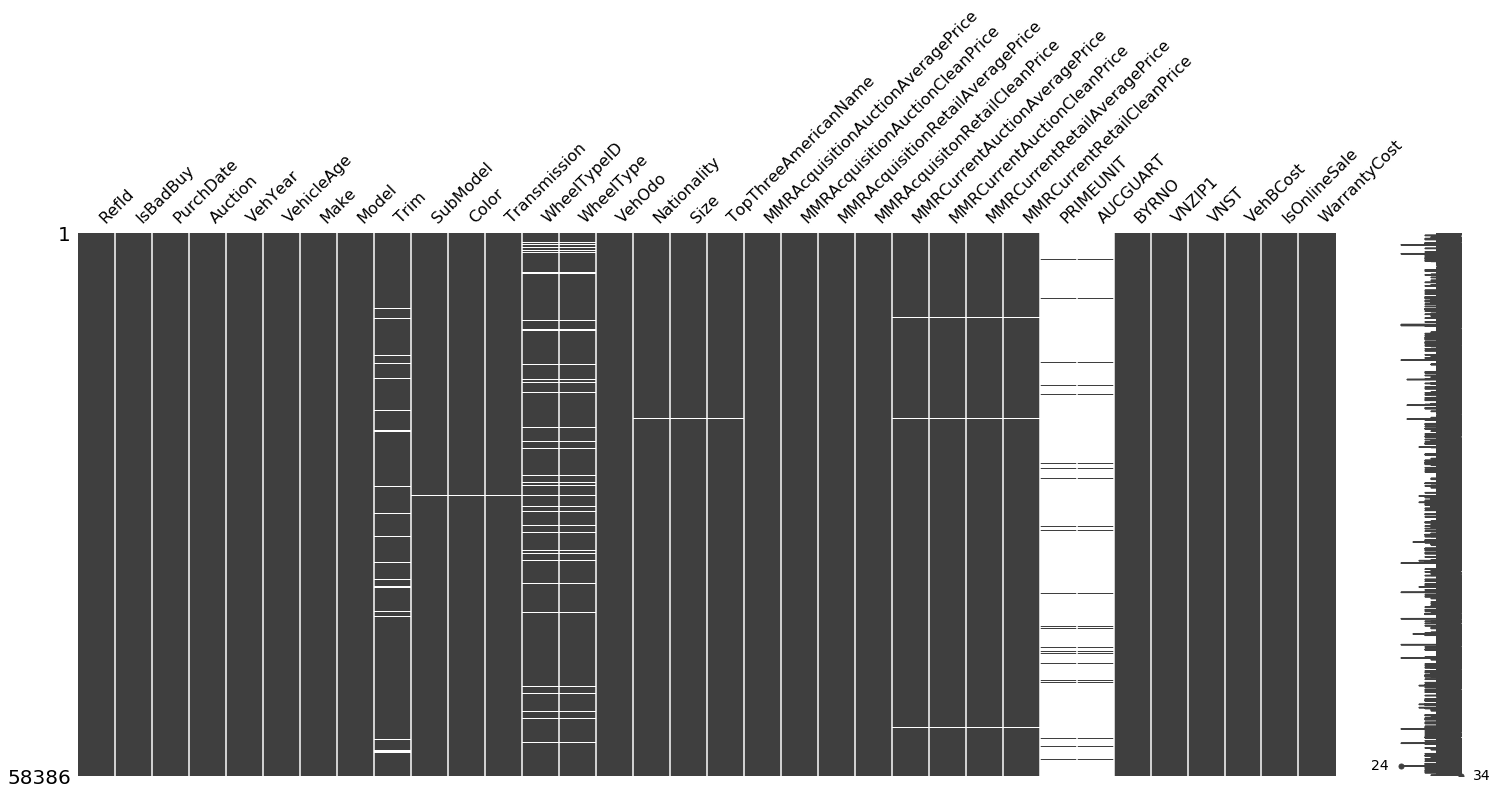
\includegraphics[width=.95\textwidth, keepaspectratio]{missingv.png}}
		\caption{{ Missing values }}
		\label{fig:missingval}
	\end{figure}
	
	With the other variables, we chose to handle the replacement in different ways depending on the meaning of each one. \\
	Some variables had very few missing values (\emph{SubModel, Color, Transmission, Nationality, Size, TopThreeAmericanName} all had $\sim 10$ missing values), therefore we replaced them using the mode. For instance, we decided to replace missing colours with the mode over groups of cars with the same model, or the transmission with the mode of the whole dataset (as almost all the cars have an automatic transmission). However, we were able to inspect manually the attributes \emph{Nationality} and \emph{TopThreeAmericanNames} and fix manually those values by just checking the car \emph{Make}.\\
	
	The main columns with missing values were the 8 \emph{MMR} prices, \emph{WheelType, WheelTypeID} and \emph{Trim}.
	We handled those cases with the following approaches:
	\begin{itemize}
		\item \emph{Trim} ($\sim 2500$ missing): we treated \emph{Trim} like the attributes discussed before. Particularly, we adopted the most frequent \emph{Trim} for a given model (or Make when given information was unavailable). In case both pieces of information were missing, we used \emph{bas} as it is the mode over all the dataset.
		\item \emph{WheelType} ($\sim 3500$ missing): We noticed that if the value of \emph{WheelTypeID} is missing, then the chance to be a bad buy highly increases (discussed in Section \ref{sec:attrDistr}, and shown in Figure \ref{fig:badbuys}). Assuming that this behaviour is meaningful, we chose to fill missing values with \emph{Unknown} and so adding a category to the attribute. Conclusively, the possible values for the \emph{WheelType} attribute became \emph{Alloy}, \emph{Covers}, \emph{Special} and \emph{Unknown}. We instead decided to drop \emph{WheelTypeID} column as it is redundant.
		\item \emph{MMR prices} ($\sim 500$ per attribute missing): we decided to handle entries with $\mathbf{price} = 0$ as if they were missing values. After that, we imputed those values using MICE (Multiple Imputation by Chained Equations) \footnote{Azur MJ, Stuart EA, Frangakis C, Leaf PJ. Multiple imputation by chained equations: what is it and how does it work?}. The new distribution is almost identical to the previous one, but of course, there is no more a peak of zeros. 
	\end{itemize}
	
	
	
	\subsection{Attributes Distribution}
	\label{sec:attrDistr}
	In this section, we will analyze the distribution of some particular attributes, showing interesting statistic plots.
	
	The first thing to note is that the target variable (\emph{IsBadBuy}), is highly imbalanced. Good buys are $87\sim88 \%$ of the population, while the remaining $12\sim13 \%$ are bad buys.
	
	In the plot shown in Figure \ref{fig:mmr}, we show the distribution of the 8 numerical attributes (before imputation) which point out the different prices of Vehicle as we explained in the first part of Data Semantics (Section \ref{sec:dataSemantics}). 
	\begin{figure}[H]
		\centering
		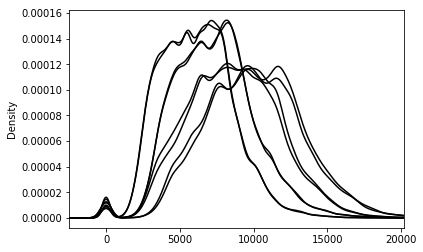
\includegraphics[width=.32\textwidth]{index}\hfill
		\includegraphics[width=.32\textwidth]{PCA1} \hfill
		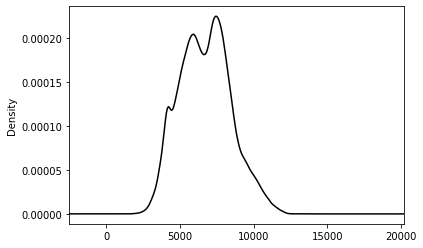
\includegraphics[width=.32\textwidth]{vehbcostNoTitle}\hfill
		\caption{Distribution (from left to right) of 8 MMR prices, PCA1 and VehBCost}
		\label{fig:mmr}
	\end{figure}
	
	We found that MMR attributes are very correlated, but the correlation is even higher when considering those prices pairwise (when considering the clean price and average price together).\\
	Furthermore, we noticed before the cleaning, the presence of a very high peak corresponding to the 0. This peak is no longer present in the variable \emph{PCA1} because, during the phase of imputation, we treated these zeros as missing values. Investigating the attribute \emph{VehBCost}, we can observe that Vehicles are usually sold for a price between 6000 and 7000, and a very low percentage of cars is sold above 11000 or below 5000 USD.
	
	
	
	\begin{figure}[H]
		\centering
		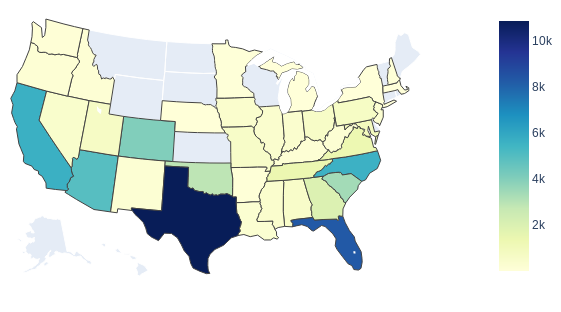
\includegraphics[width=.65\textwidth]{newplot.png}
		\caption{{ Distribution of the attribute VSNT}}
	\end{figure}
	
	To improve the understanding of the attribute \emph{VSNT}, we plotted this variable on the map of the United States. The figure is suggesting that Texas is the state with most of the auctions (18800), followed by Florida (8317) and California (5673). On the other hand, the state with the lower number of auctions is New York (4). Interestingly enough, there are no auctions in Montana, Wyoming, North Dakota, South Dakota, Kansas, Wisconsin, Maine, Vermont, Rhode Island and Connecticut.
	
	\begin{figure}[H]
		\centering
		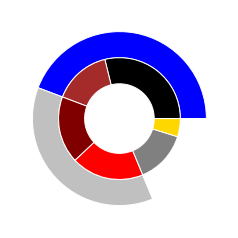
\includegraphics[width=.3\textwidth]{color.png}
		\caption{Distribution of the attribute Color}
		\label{fig:color}
	\end{figure}
	
	
	As far as the attribute \emph{Color} concerns (Figure \ref{fig:color}), it is not surprising that the most common colours are blue, silver and white. We also tried to plot colours along with other categorical attributes like \emph{VehicleYear} or \emph{Make}, but unfortunately, as Figure \ref{fig:colorwrt} shows, we discovered that this attribute is independent of the others, in fact, its distribution does not change almost at all.
	
	
	\begin{figure}[]
		\centering
		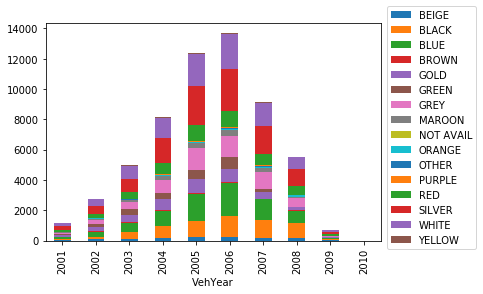
\includegraphics[width=.5\textwidth, keepaspectratio]{barcoloryear.png}\hspace{1cm}
		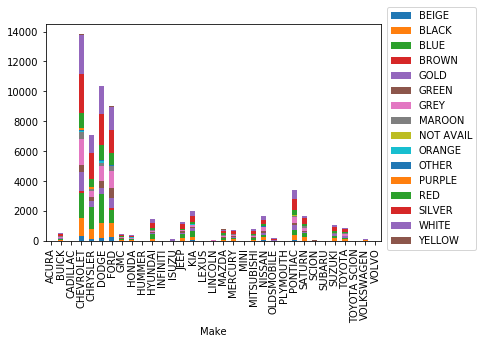
\includegraphics[width=.42\textwidth, keepaspectratio]{barcolormake.png}
		\caption{Color attribute plotted w.r.t vehicle year and make}
		\label{fig:colorwrt}
	\end{figure}
	
	
	Afterwards, we inspected the variable \emph{IsBadBuy}. In Figure \ref{fig:badbuys} (on the left), we first put \emph{WarrantyCost} and \emph{VehOdo} in relationship. The most interesting point was that bad purchases are more frequent in less dense areas. Whereas when we dealt with \emph{WheelType} (on the right), we noticed that the number of bad buys is huge whenever the information is lacking (corresponding to the column labelled as \emph{Unknown}).
	
	
	\begin{figure}[H]
		\centering
		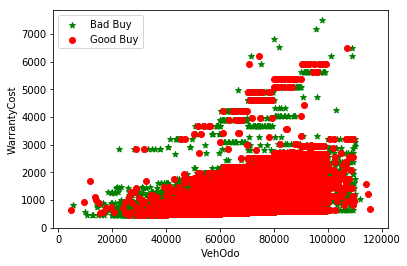
\includegraphics[width=.4\textwidth, keepaspectratio]{badbuys} \hspace{1cm}
		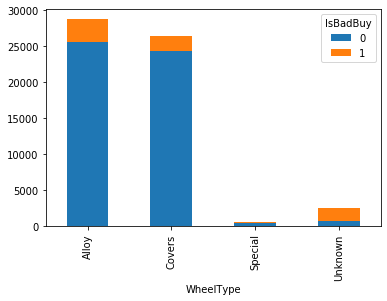
\includegraphics[width=.33\textwidth, keepaspectratio]{wheeltype}
		\caption{IsBadBuy distribution with respect to VehOdo and VehBCost}
		\label{fig:badbuys}
	\end{figure}
	
	Next, in Figure \ref{fig:fantastic}, we emphasise that each car manufacturer belongs to a precise price range and, more importantly, the warranty costs change a lot among them. Note that the size of the circles describes the number of cars belonging to that manufacturer. We understood that the \emph{Top Three American Names} (namely Ford, General Motors and Chrysler) hold the great majority of sales. Their cost is usually close to the average, but the warranty cost is pretty high compared to Japanese cars. Furthermore, Hummer is by far the most costly car, while Suzuki has the best quality/price ratio.
	
	
	\begin{figure}[H]
		\centering
		\captionsetup{justification=centering}
		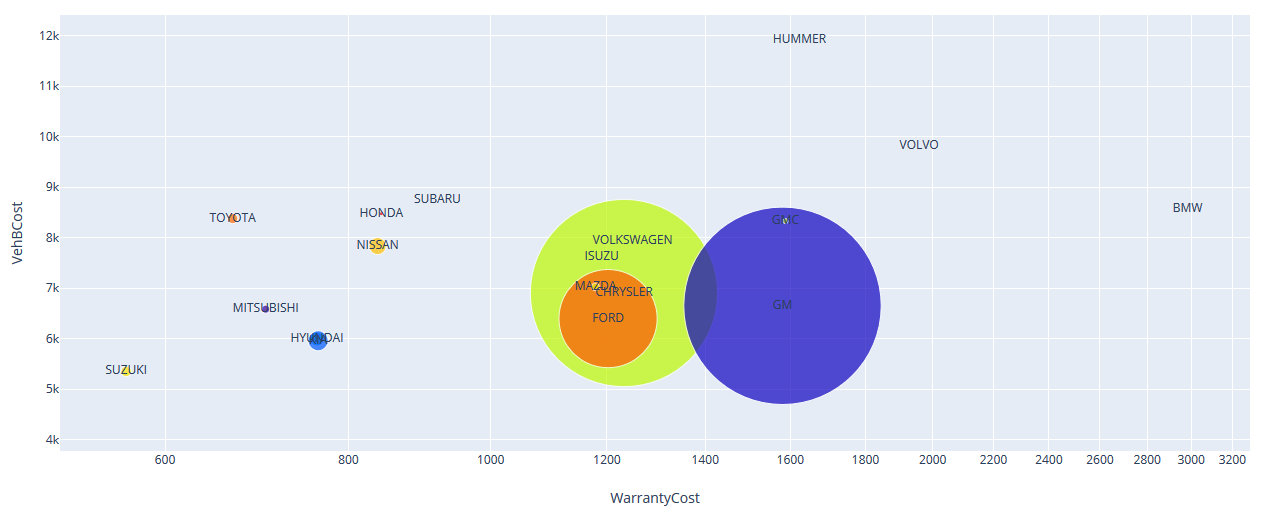
\includegraphics[width=.95\textwidth, keepaspectratio]{fantastic.png} 
		\caption{Distribution of \emph{Make} w.r.t the cost and the warranty cost. The diameter of each circle represents the frequency of that make in the dataset.}
		\label{fig:fantastic}
	\end{figure}
	
	\newpage
	\section{Clustering}
	\label{sec:clustering}
	In this section, we describe the three Clustering algorithms applied to the data set (KMeans, DBScan and Hierarchical), and their results.
	
	\subsection{Function Selection}
	In K-means we tried to use both the \emph{MinMax} scaler and the standard \emph{z} scaler, observing that the clustering results were very similar. In the end, we chose to use the MinMax one. 
	In DBScan and Hierarchical, instead, we adopted the Standard one because it gave us slightly better results
	
	\subsection{KMeans}
	The following sections present the analysis of the results of the KMeans clustering algorithm.
	
	\subsubsection{Attributes' selection}
	Considering that our dataset contains information about car auctions, we opted to study characteristics about cars, like the amount of kilometers the car has done (\textbf{VehOdo}), the auction selling price for said car (\textbf{VehBCost}), the cost of repairing or replacing previously sold products (\textbf{WarrantyCost}) and some samples of the different prices (i.e. \textbf{AAAP, ARAP}).
	
	We built 5 Dataframes with these attributes to study which was the best combination of them.
	
	\begin{table}[H]
		\centering
		\begin{tabular}{|c|c|}
			\hline
			& Attributes set \\
			\hline
			\rowcolor{Gray}
			1 & VehOdo,  VehBCost,  AAAP \\
			2 & WarrantyCost, VehBCost ,  AAAP  \\
			\rowcolor{Gray}
			3 & AAAP,  ARAP ,  VehBCost \\
			4 & WarrantyCost,  VehOdo,  VehBCost  \\
			\rowcolor{Gray}
			5 & WarrantyCost,  AAAP, VehOdo \\
			\hline
		\end{tabular}
	\end{table}
	
	
	\subsubsection{Identification of best k}
	
	
	In order to pick the best parameter k for K-Means, we made use of the Knee method by computing the SSE for k $\in$ [2,16]. The best SSE was obtained in the Data Frame 3, which was originally chosen for its high correlation among the attributes.
	
	However, when we tried plotting the data, we did not obtain any interesting information in order to better interpreter the data behaviour. We then decided to give up the best SSE by choosing the Data Frame 4 which has a lower SSE but semantically more interesting results.
	
	
	\begin{figure}[H]
		\centering
		\includegraphics[width=.49\textwidth]{cattura}\hfill
		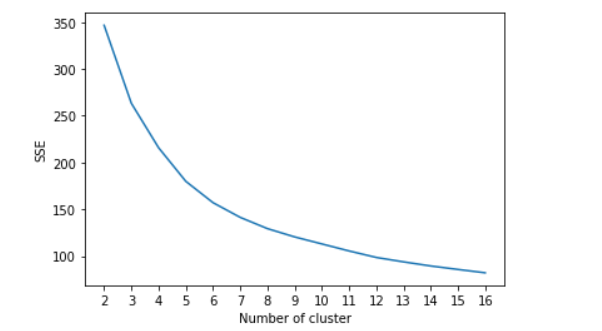
\includegraphics[width=.49\textwidth]{SSE2}
		\caption{Plot SSE of Attribute set 3 (left) and 4 (right).}
		\label{fig:KmeansSSE}
	\end{figure}
	We noticed that the SSE curves for all the data frames share a strong similarity (same curvature, but different SSE). Indeed their behaviours are very close to the ones shown in Figure \ref{fig:KmeansSSE}.
	Then we discovered ,using the \emph{knee method}, that the best value for all the data frames was \emph{k = 6}. A comprehensive analysis of all the data frames is shown in Table \ref{tab:SSESilu}. In particular, the lowest SSE is by far the one of data frame 3.\\
	However, we decided to discard this result since the 6 clusters found by the algorithm were essentially groups of cars in different price ranges. We decided that the best clustering, both semantically and parameter wise, was DF4 (the one taking in consideration \emph{WarrantyCost, VehOdo and VehBCost}).
	
	\begin{table}[H]
		\centering
		\begin{tabular}{|c|ccc|}
			\hline
			&  Best k & SSE& Silhouette \\
			\hline
			\rowcolor{Gray}
			DF1 & 6 & 106.0 & 0.309 \\
			DF2 & 6 & 90.0 & 0.307  \\
			\rowcolor{Gray}
			DF3 & 6 & 40.0 & 0.294 \\
			DF4 & 6 & 157.0 & 0.287  \\
			\rowcolor{Gray}
			DF5 & 6 & 184.0\textbf & 0.278 \\
			\hline
		\end{tabular}
		\caption{{Summary of the SSE, Silhouette and k values obtained for all the Attribute sets with K-means}}
		\label{tab:SSESilu}
	\end{table}
	
	
	\subsubsection{Description of the best clustering}
	\label{sec:clusterdescr}
	The following descriptions refer to the results of the clustering that were proposed as the best in the previous section. Every result is presented with its centroid, that describes the core point of the cluster, and a textual interpretation of the kind of cars that are present in those clusters. 
	The centroids coordinates are expressed like this:  
	$$ \mathbf{centroid} = (\mathbf{VehBCost}, \mathbf{WarrantyCost}, \mathbf{VehOdo}) $$
	In Figure \ref{fig:centroid} the clustering results are shown plotted in 2 dimensions (\emph{WarrantyCost} and \emph{VehOdo}). The plot does not show the third dimension (\emph{VehBCost}) because this latter is the least important feature (as it will be evident from the centroids shown when describing the clusters in Section \ref{sec:clusterdescr}).
	The figure also shows the cluster centroids with a star on the plot. 
	
	\begin{figure}[H]
		\centering
		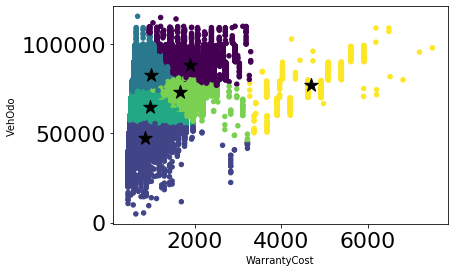
\includegraphics[width=.7\textwidth, keepaspectratio]{centroid}
		\caption{{Clusters plotted with WarrantyCost and VehOdo}}
		\label{fig:centroid}
	\end{figure}
	
	
	The clusters descriptions for Figure \ref{fig:centroid} are:
	\begin{enumerate}
		\item $\mathbf{centroid}: (6\,500,  1\,900,  88\,000)$: cars with very high odometer reading and pretty high warranty cost (purple cluster). Those cars are sold for a price which is in line with the mean of the prices.
		\item $\mathbf{centroid}: (6\,800,  850,  48\,000)$: cars which are pretty new , with low  reading and low warranty cost (light blue cluster). As expected their cost is slightly above average.
		\item $\mathbf{centroid}: (6\,400,  1\,000,  83\,000)$: cars with high odometer reading but low warranty cost (azure cluster). Those cars are probably considered to be solid (low outage risk) even after years of use, and are sold at a normal price.
		\item $\mathbf{centroid}: (6\,700,  1\,000,  65\,000)$: cars with low warranty cost and average odometer (aquamarine cluster). There is not much to say about this cluster, as it represents the average car.
		\item $\mathbf{centroid}: (7\,300,  1\,700,  73\,000)$: Cars with high warranty cost, but average odometer reading (green cluster). This is one of the most interesting clusters, as it shows that relatively high-risk cars are sold at a price which is higher than expected (considering high warranty cost as a sign of risk).
		\item $\mathbf{centroid}: (5\,300,  4\,700,  77\,000)$: Exceptionally high warranty cost, high odometer reading (yellow cluster). This cluster is the least populated and the most sparse one. It homes those very risky buys, and in addition to that, cars in this cluster are also pretty dated. They are sold, as expected, at a very low price. 
	\end{enumerate}
	Given these outcomes, we tried to understand if bad buys were located mainly in one of those clusters. By plotting this information in Figure \ref{fig:clusterbuy}, we noticed that cluster 2 (new cars with low odometer reading), has the least amount of bad buys.
	\begin{figure}[H]
		\centering
		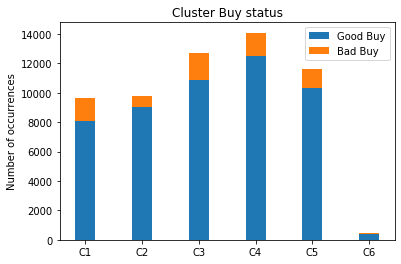
\includegraphics[width=.4\textwidth, keepaspectratio]{clusterbuy}
		\caption{{Distribution of IsBadBuy with respect to the 6 clusters found}}
		\label{fig:clusterbuy}
	\end{figure}
	
	\subsection{DB Scan}
	In this section, we explain the approach used to generate clusters with DBscan algorithm.
	
	\subsubsection{Attributes and distance function}
	We decided to follow the same reasoning used for \emph{KMeans}, thus we attempted to do the clustering over the same set of attributes. We also chose to use Euclidean distance, and Z-Score scaling.
	
	The results shown in the following sections are only relative to the data frame with columns \emph{VehOdo, VehBCost} and \emph{WarrantyCost} (the same data frame used for KMeans). Other possible attributes choices did not change much the final result, so we decided that using the same attributes allows us to more easily see the difference between the two algorithms.
	
	
	\subsubsection{Study of the clustering parameters}
	In order to choose the right $\epsilon$ and $\mathbf{min points}$, we adopted the knee method by plotting the distance to the \emph{k-th} nearest neighbour, where k was taken from [32, 64, 128, 256, 512]. The resulting curves, shown in Figure \ref{fig:kth}, were used to select the right epsilon for attempting the clustering with DB-Scan. 
	
	\begin{figure}[]
		\centering
		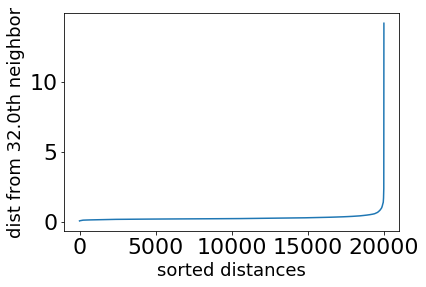
\includegraphics[width=.32\textwidth]{a32}\hfill
		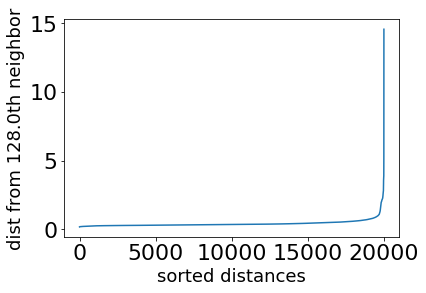
\includegraphics[width=.32\textwidth]{a128}\hfill
		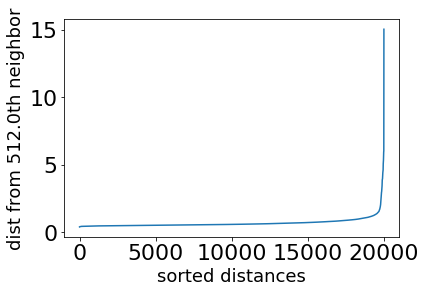
\includegraphics[width=.32\textwidth]{a512}
		\caption{k-th neighbour distance, with k = 32, k = 128, k = 512}
		\label{fig:kth}
	\end{figure}
	
	Given those plots, we chose epsilon as shown in Table \ref{tab:kth}.
	It is important to know, however, that this approach failed for reasons described in Section \ref{sec:dbscaneval}, so another set of attributes with more interesting results is shown in Table \ref{tab:dbscan}. Those values were found by brute force, by attempting, for all k shown in the list before, $\epsilon = 0.1, 0.11, 0.12\dots 0.8$, and visually inspecting the results.\\
	
	\begin{table}
		\parbox{.45\linewidth}{
			\centering
			\begin{tabular}{|c|c|}
				\hline
				min points & $\epsilon$\\
				\hline
				\rowcolor{Gray}
				32 & 0.75 \\
				64 & 0.95 \\
				\rowcolor{Gray}
				128 & 1.22 \\
				256 & 1.36 \\
				\rowcolor{Gray}
				512 & 1.64 \\
				\hline
			\end{tabular}
			\caption{K-th nearest neighbours parameters}
			\label{tab:kth}
		}
		\hfill
		\parbox{.45\linewidth}{
			\centering
			\begin{tabular}{|c|c|}
				\hline
				min points & $\epsilon$\\
				\hline
				\rowcolor{Gray}
				32 & 0.17 \\
				64 & 0.22 \\
				\rowcolor{Gray}
				128 & 0.29 \\
				256 & 0.38 \\
				\rowcolor{Gray}
				512 & 0.48 \\
				\hline
			\end{tabular}
			\caption{Manually found parameters}
			\label{tab:dbscan}
		}
	\end{table}
	
	\subsubsection{Characterization and interpretation of the obtained clusters}
	\label{sec:dbscaneval}
	First, we are going to analyze the results with parameters shown in Table \ref{tab:kth}. The algorithm produced as a result a single cluster containing all the points in the data set, with the exception of $\sim 100$ elements, which were labelled as noise points. The main reason was that the data forms one big cloud of points, with different density distributions inside. This kind of behaviour represents the conditions under which DB scan performs worst, and this is the reason why the \emph{k-th} neighbour distance approach failed. \\
	We then decided to try and find the densest areas in the data set, by manually checking a lot of parameters configurations. This approach, however, does not find any cluster, but it only finds highly populated areas in the data set. 
	The best results were found when the number of noise points was close to half the total amount in the data set. Those results correspond to the ones found with the parameters shown in Table \ref{tab:dbscan} and some example of such clustering is shown in Figure \ref{fig:dbscan}.
	
	\begin{figure}[H] 
		\centering
		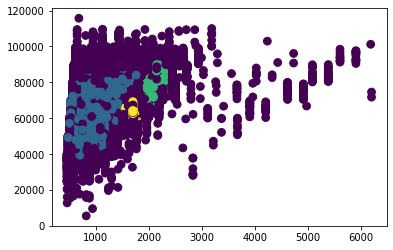
\includegraphics[width=.40\textwidth]{cazzo}\hspace{1cm}
		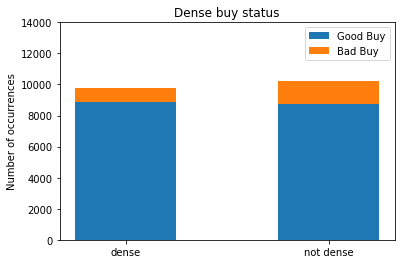
\includegraphics[width=.4\textwidth]{bigboi}
		\caption{DBScan clustering results with $\mathbf{minpoints} = 256$ and $\epsilon = 0.38$. Purple colors are noise points}
		\label{fig:dbscan}
	\end{figure}
	
	We realised that most of the cars have $50\,000 \sim 70\,000$ odometer reading when sold, and denser areas contain less bad buys overall. \\
	In general, DBscan is the algorithm that performs the worst on this data set.
	
	\subsection{Hierarchical Clustering}
	In this section, we explain the approach used to generate clusters with Hierarchical algorithm.
	\subsubsection{Attribute Choices}
	We decided to perform clustering on the following attributes set:
	\begin{enumerate}
		\item \emph{VehOdo, VehBCost, AAAP}
		\item \emph{WarrantyCost, VehBCost, VehOdo}
	\end{enumerate}
	
	\subsubsection{Algorithms and Dendrograms}
	\label{sec:hier}
	We decided to perform hierarchical clustering with Euclidean and Manhattan distance as metrics, and to perform, for each of those metrics ward, single, complete and average linkages (with the exception of Manhattan distance with ward linkage, being it not allowed).\\
	For each one of those results, we attempted clustering with $\mathbf{numberOfCluster} \in [2, 10]$, and computed the silhouettes for all the results.
	Figure \ref{fig:silu} shows the silhouettes for the results found with all the algorithms on data frame 2 (the same used for KMeans and DBScan).
	\begin{figure}[]
		\centering
		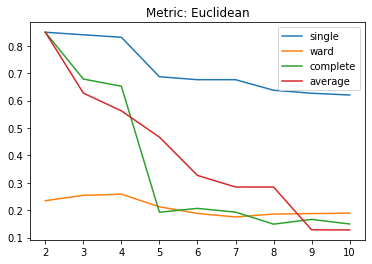
\includegraphics[width=.35\textwidth]{silueuc}\hspace{1cm}
		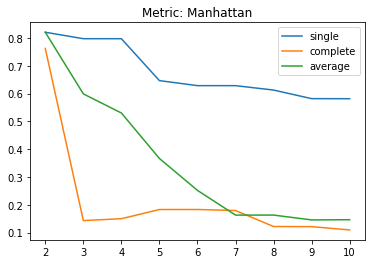
\includegraphics[width=.35\textwidth]{siluman.png}
		\caption{Silhouettes for all algorithms and all metrics on data frame 2}
		\label{fig:silu}
	\end{figure}
	From those plot, we notice a tendency for the silhouette to drop when the number of cluster passes from 4 to 5. We then decide to perform clustering with 4 clusters.
	Given that, we visually inspected the results and found that the only ones with interesting clusters are:
	\begin{itemize}
		\item Euclidean metric and ward linkage
		\item Manhattan metric and complete linkage
	\end{itemize}
	The visual result of those clustering is shown in Figure \ref{fig:hier}, while their respective dendrograms are shown in Figure \ref{fig:dend}. All the other clustering attempts produced highly imbalanced cluster (one main cluster and some single digit size clusters).
	\begin{figure}[H]
		\centering
		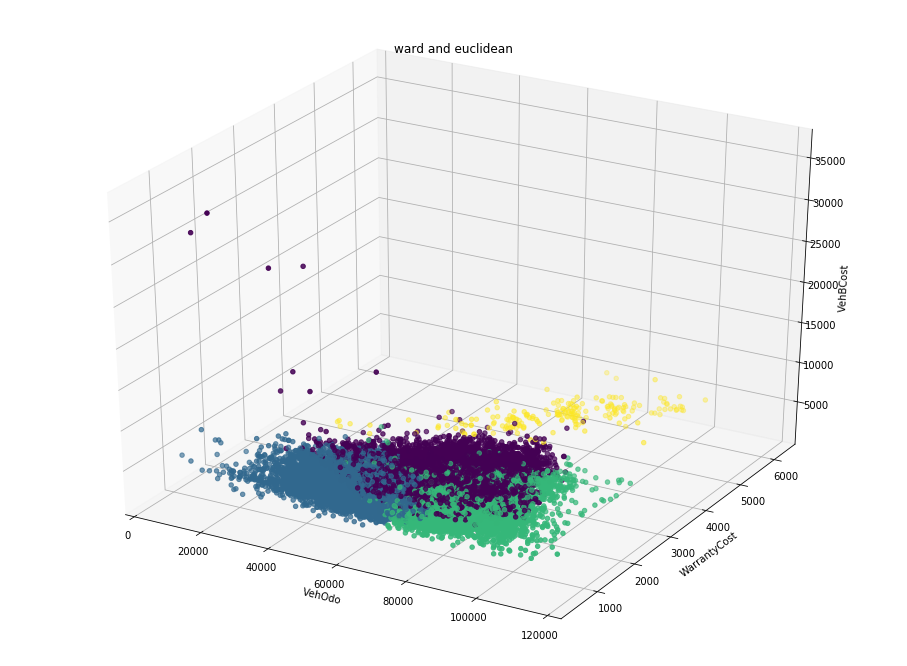
\includegraphics[width=.44\textwidth]{wardeucl}\hspace{1cm}
		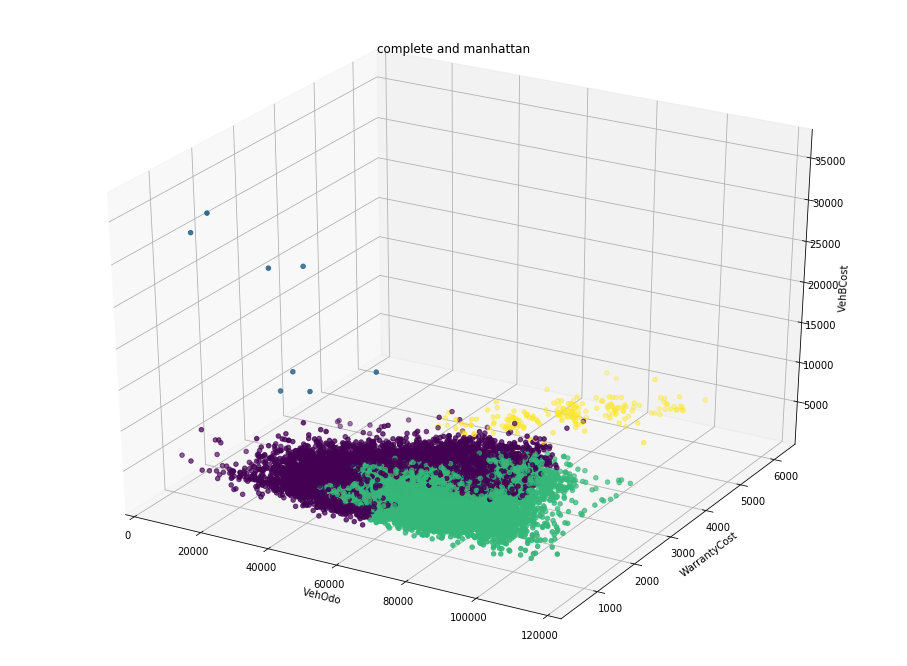
\includegraphics[width=.44\textwidth]{complman}
		\caption{Hierarchical clustering results, number of clusters is 4}
		\label{fig:hier}
	\end{figure}
	\begin{figure}[H]
		\centering
		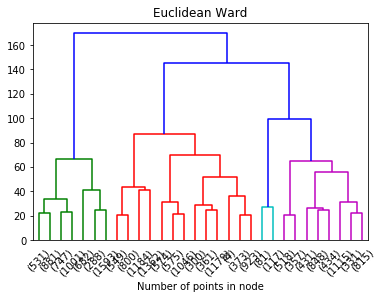
\includegraphics[width=.44\textwidth]{dendeuc}\hspace{1cm}
		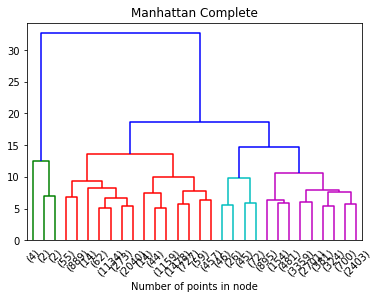
\includegraphics[width=.44\textwidth]{dendman}
		\caption{Dendrograms plotted with \emph{lastp} truncate mode}
		\label{fig:dend}
	\end{figure}
	
	
	\subsubsection{Best clustering approach and comparison of the clustering obtained}
	In conclusion, the best clustering results were found in the circumstances shown in Section \ref{sec:hier}. The results, semantically speaking, highly resemble the ones found using KMeans.\\ Both results find a cluster in the high warranty cost cars (displayed in both Figure \ref{fig:hier} and in Figure \ref{fig:centroid} for KMeans, where the highlighted cluster is displayed in yellow).\\
	The main difference is in the way that points in the "big cloud" are assigned a cluster. The reasoning, anyway, is really similar to the one made in Section \ref{sec:clusterdescr} regarding KMeans, so we refer to that one.
	
	
	
	\newpage
	\section{Classification}
	\label{sec:classification}
	In the following section, we describe the methodologies and the algorithms used during the classification. The main goal of this task was to predict the variable called \textit{IsBadBuy}, that indicates whether a car has been a good business or not.
	
	\subsection{Hyper-parameters Optimization}
	To discover the best way to predict the required variable, we tested a lot of models by optimizing their hyper-parameters. Those act as knobs to fine-tune the model, so to provide the best result, we need to find out the optimal value of these parameters, or in other words, a trade-off between true/false positives and true/false negatives. Since each algorithm has its peculiarity, for each classificator, we created different groups of parameters to experiment. Table \ref{tab:hyper} shows the setup of our analyses.
	
	
	\begin{table}[H]
		\begin{center}
			\begin{tabular}{| c | c |}
				\hline
				\textbf{Algorithm} & \textbf{Hyper-parameters}\\
				\hline
				\rowcolor{Gray}
				Random Forest & \textit{n\_estimators}: 25, 50, 100, 200, 500, 1000 \\
				\hline
				Decision Tree & \specialcell{
					\textit{criterion} : 'gini', 'entropy'\\
					\textit{max\_depth} : 2, 5, 10, 15, None\\
					\textit{min\_samples\_split} : 2, 5, 10, 20}\\
				\hline
				\rowcolor{Gray}
				AdaBoost & \specialcell{
					\textit{n\_estimators} : 5, 10, 25, 50, 100 \\
					\textit{learning\_rate} : 0.1, 0.25, 0.5, 0.75, 1} \\
				\hline
				KNN & \specialcell{
					\textit{n\_neighbors} : 1, 4, 7, 10, 13, 16, 19, 22, 25, 28 \\
					\textit{weights} : 'uniform', 'distance' } \\
				\hline
			\end{tabular}
		\end{center}
		\caption{Setup environment of the tested hyper-parameters}
		\label{tab:hyper}
	\end{table}
	
	
	\subsubsection{Methodology}
	The first step was to isolate the test set ("test.csv") because this will be used as ground truth to verify the performance of the final models. Then, we cross-validate each model by using as input data, the given training set ("training.csv"). To reflect the percentage of the initial datasets, we decided to split the data in 60-40 (respectively training and validation). For each algorithm of classification, and for each tuple of parameters, we performed 5 Cross-Validation and we averaged the results to circumvent overfitting/underfitting. Do note that to improve the classes imbalance, undersampling and oversampling techniques have been applied.
	
	\subsection{Results}
	The following pictures show the performance obtained by each algorithm during the optimization. Our strategy was to focus more on optimizing Recall and F1 because our goal was to discover "bad buys". The yellow dots/squares represent our best choice of hyper-parameters. Overall the most suitable classifier for this task were decision trees and random forest.
	
	\subsubsection{Random Forest}
	\begin{figure}[H]
		\centering
		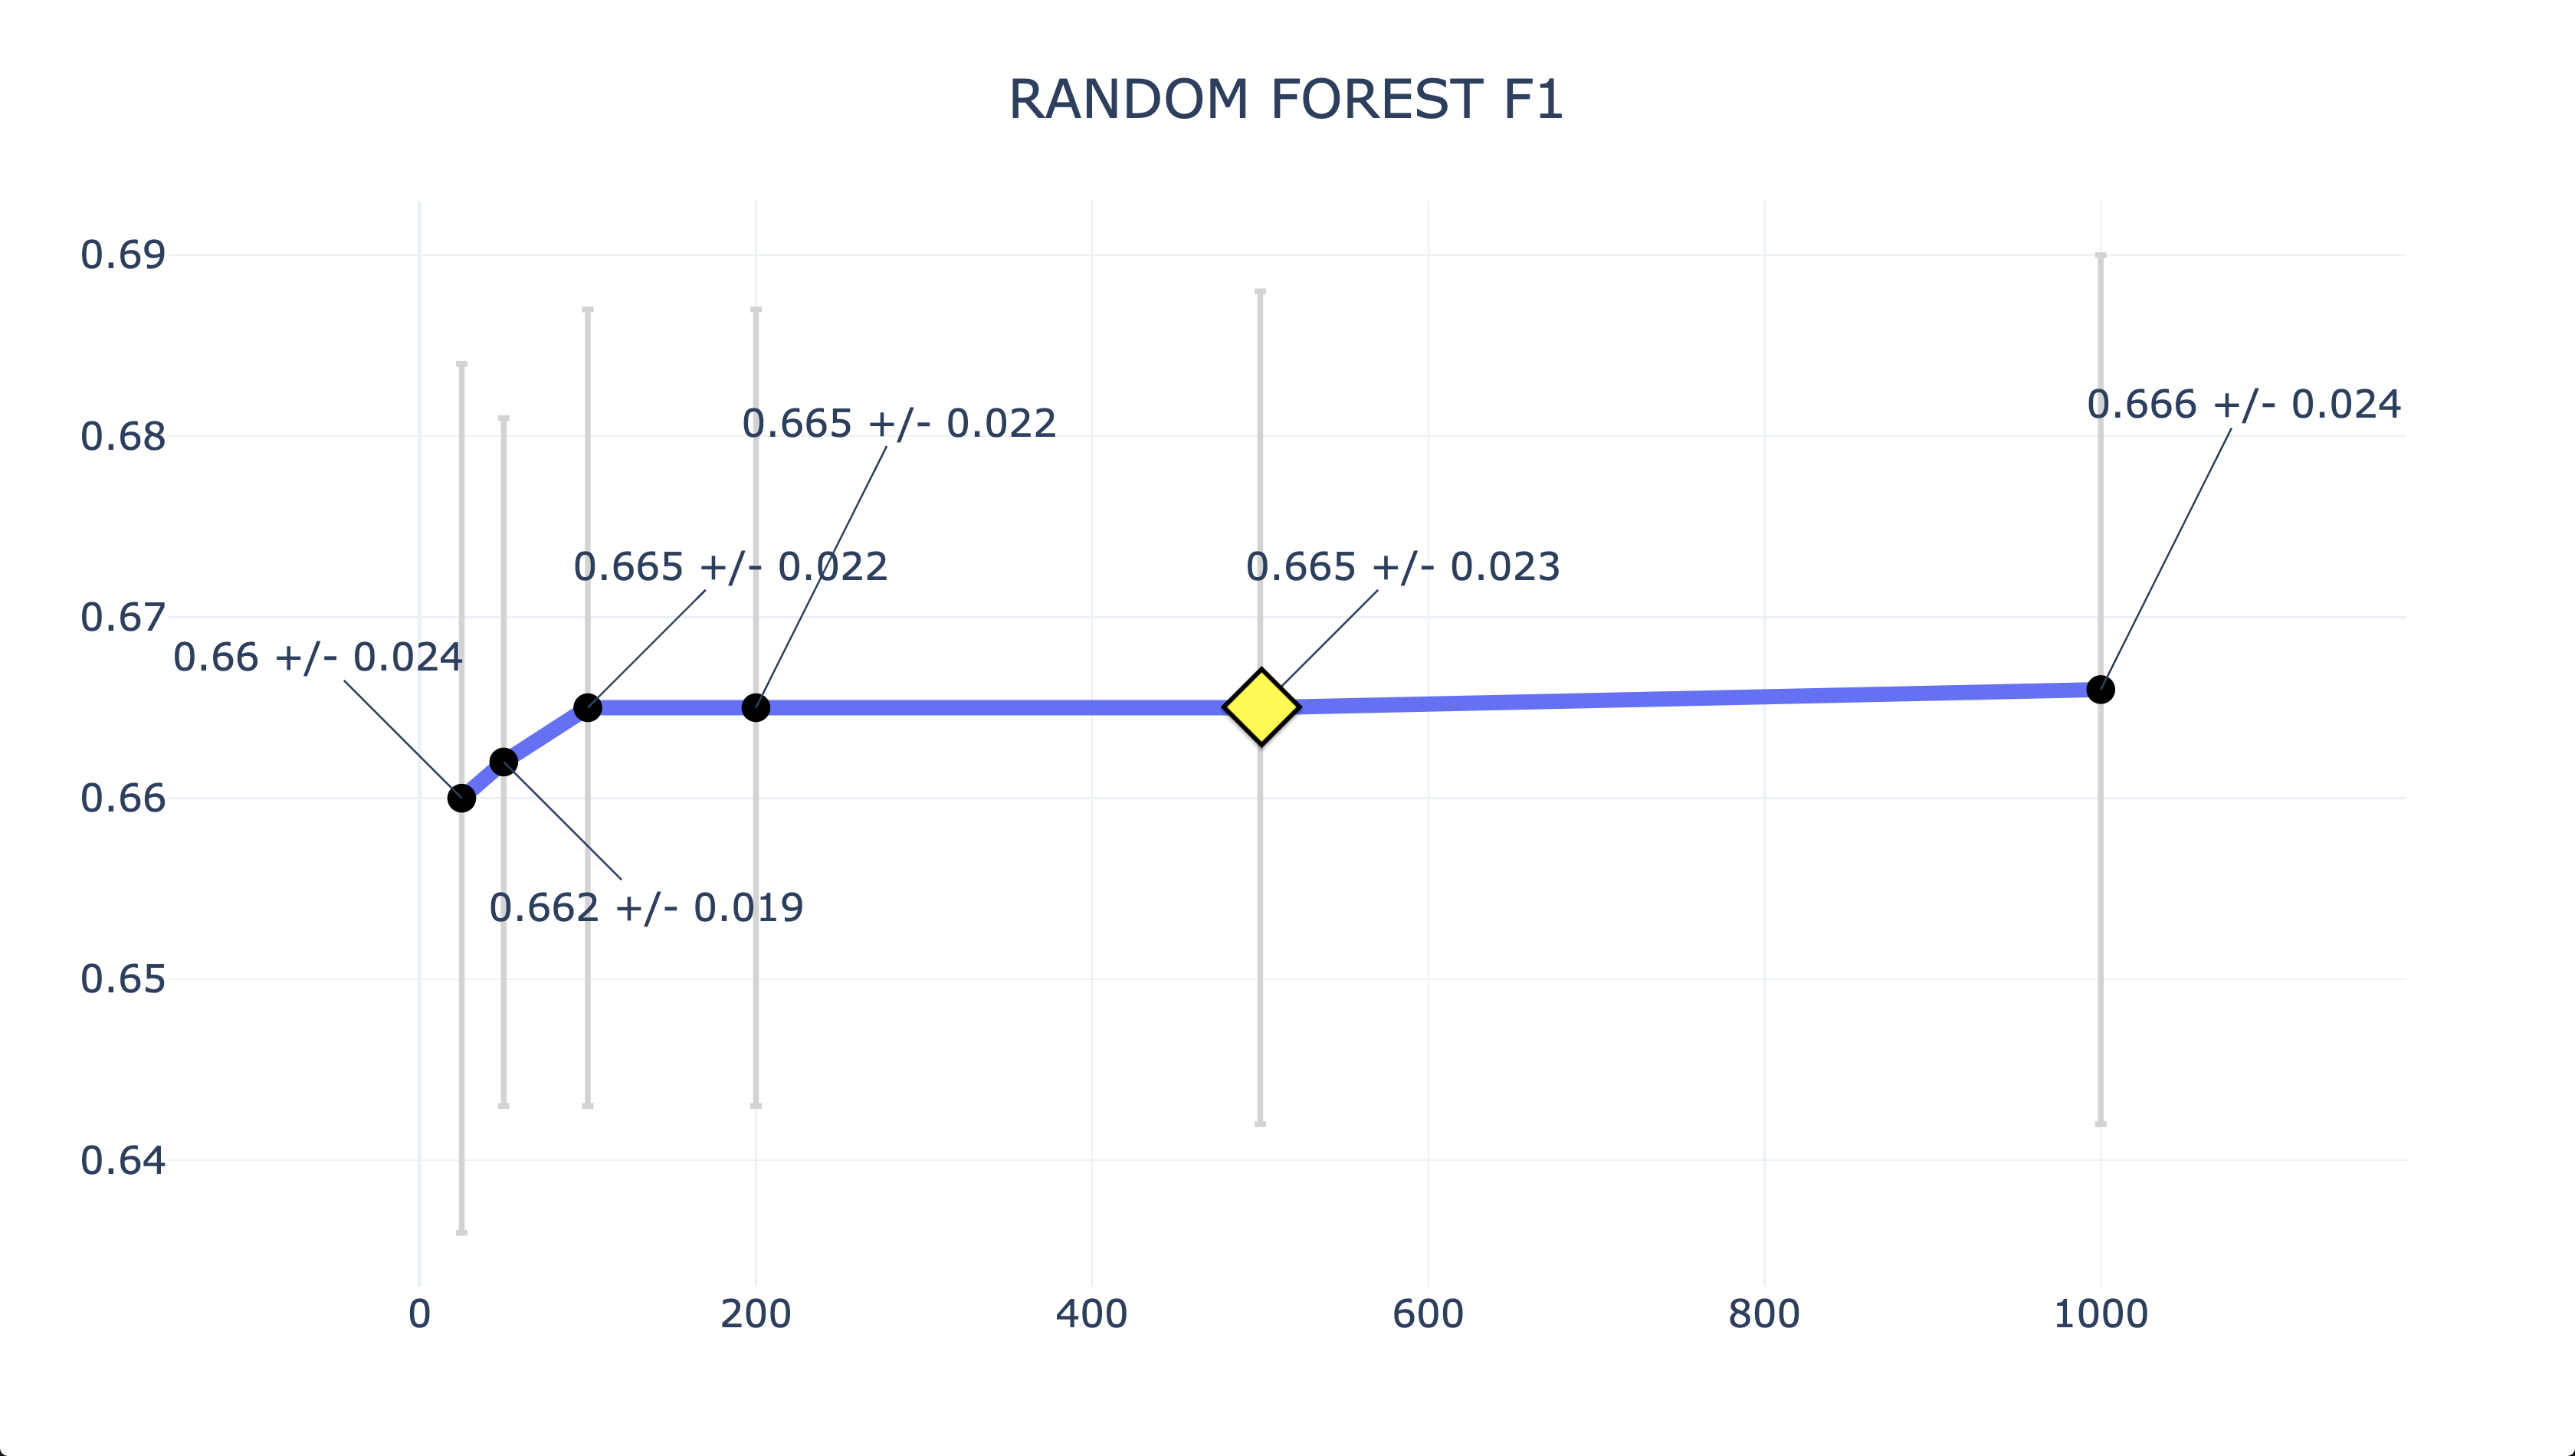
\includegraphics[width=.45\textwidth]{clf_img/RF_f1.png}
		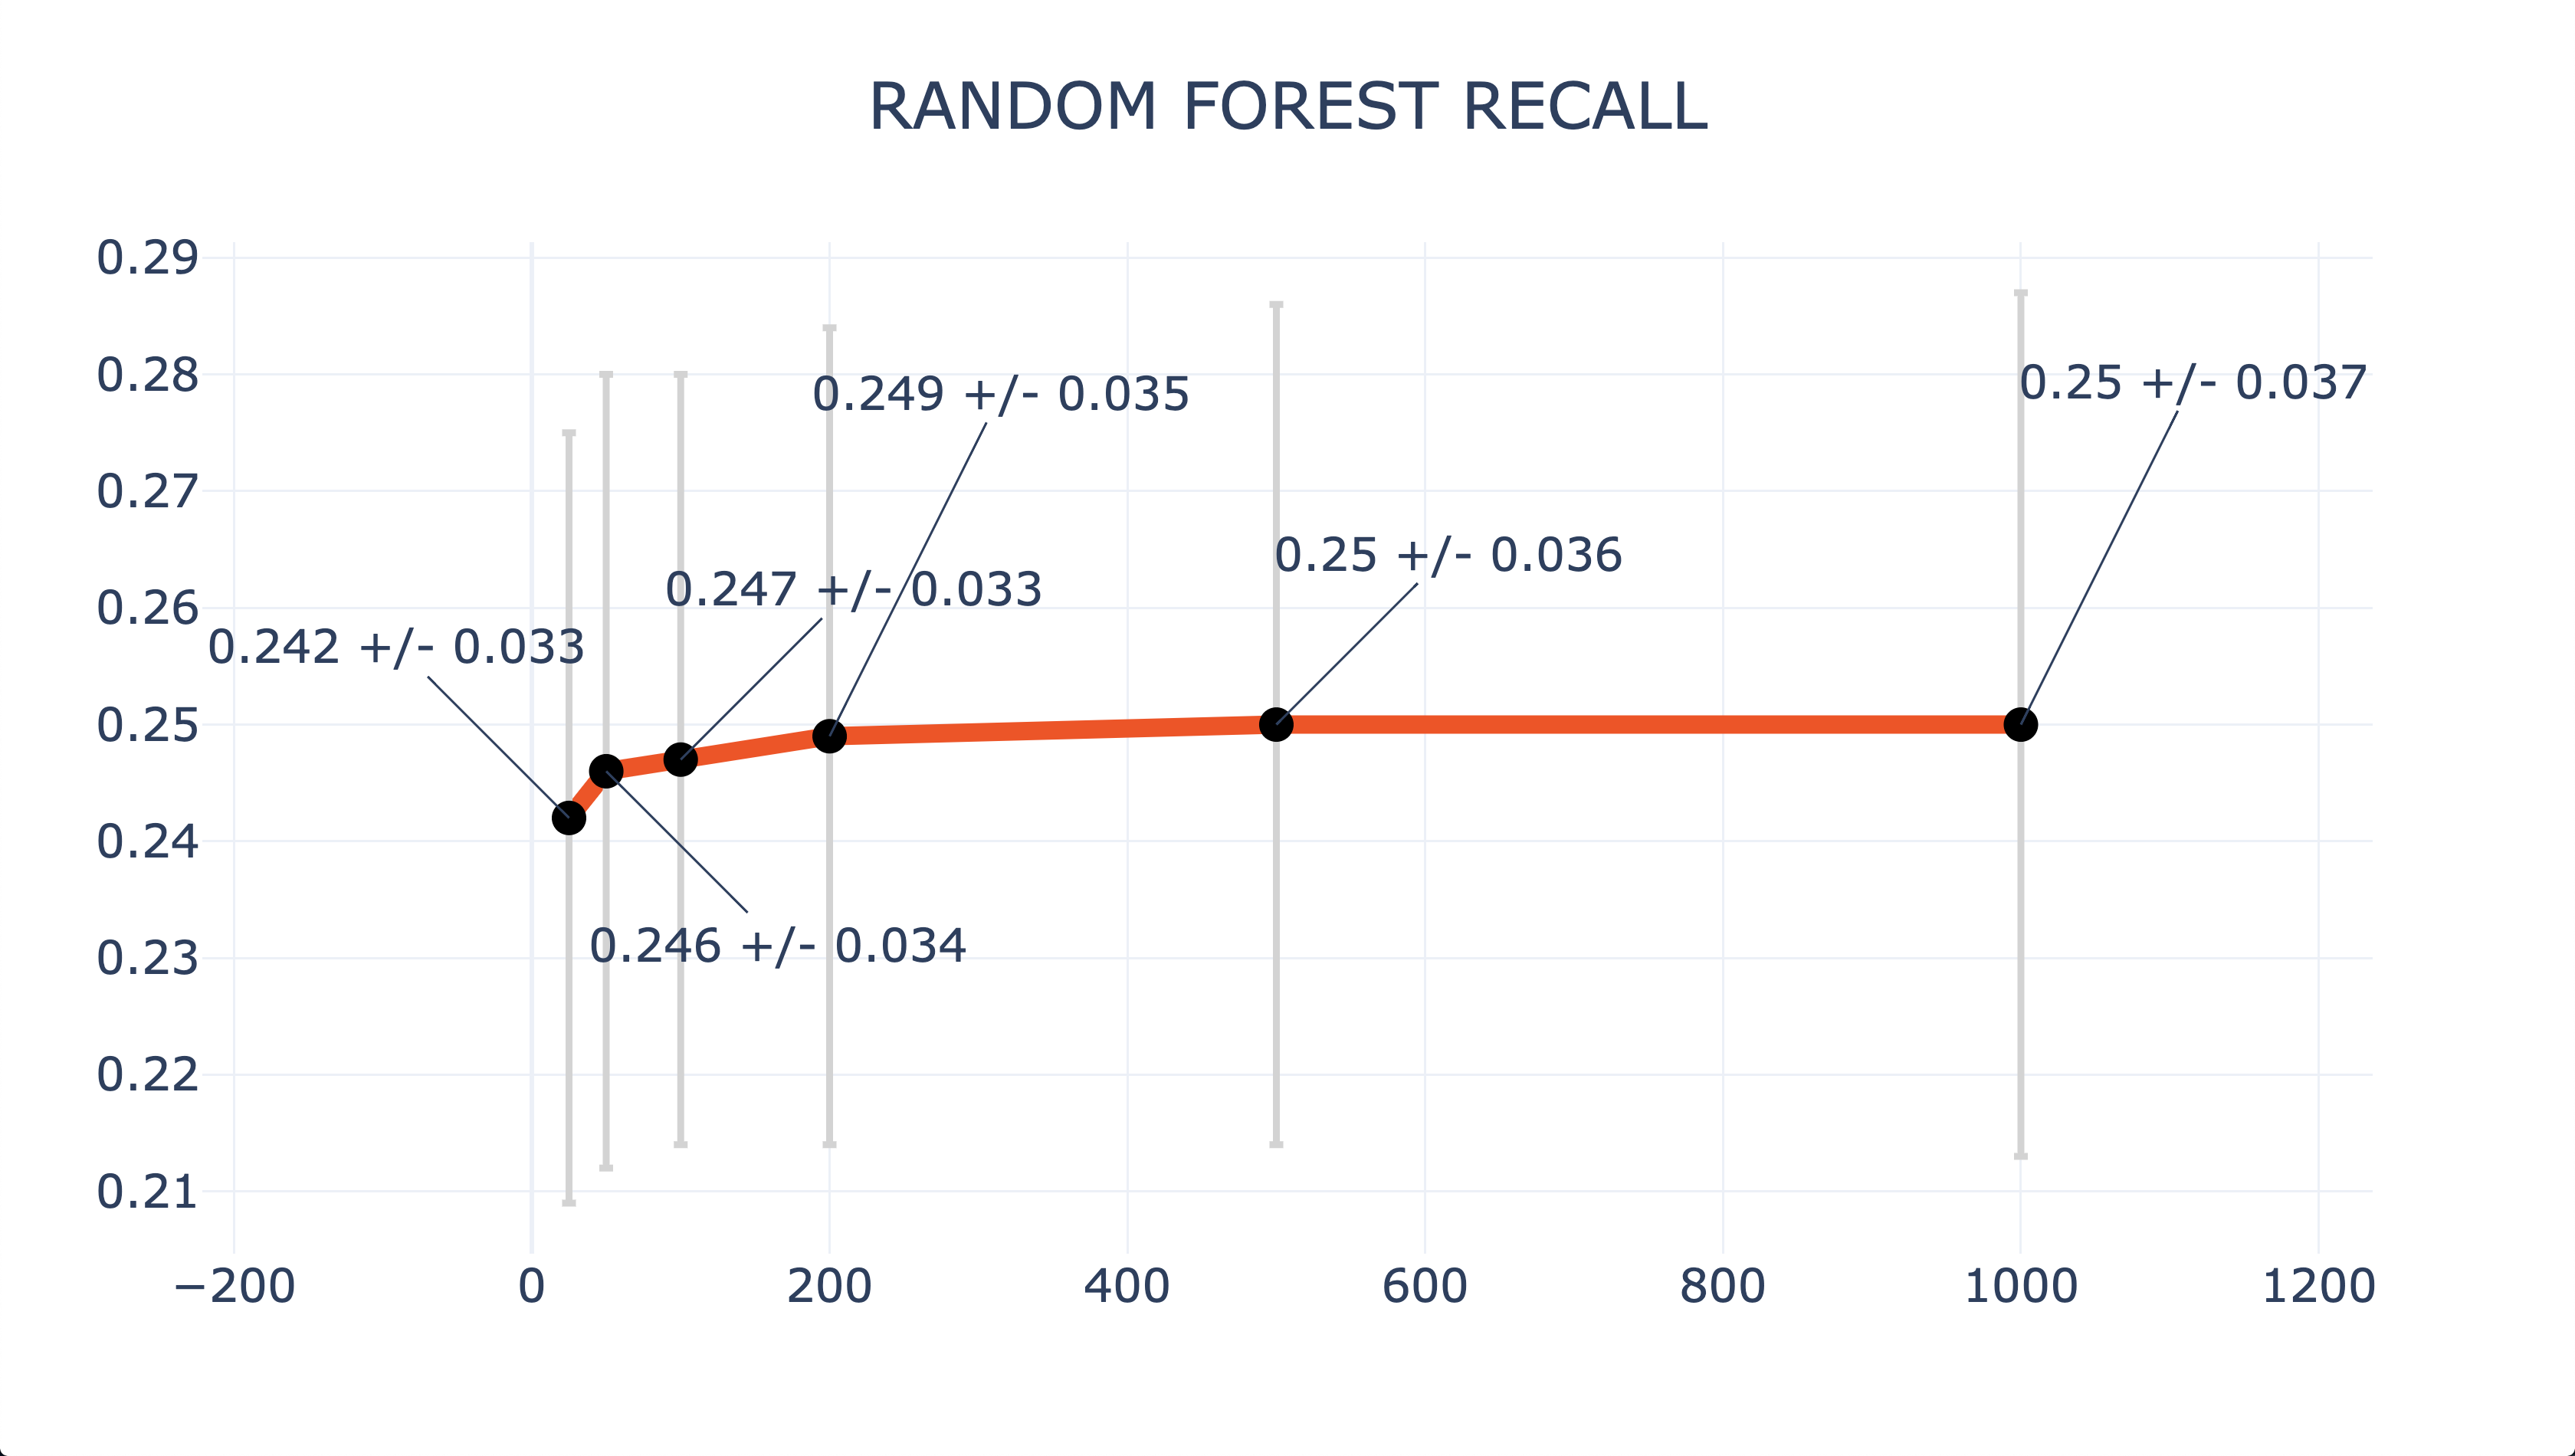
\includegraphics[width=.45\textwidth]{clf_img/RF_recall.png}
	\end{figure}
	\begin{figure}[H]
		\centering
		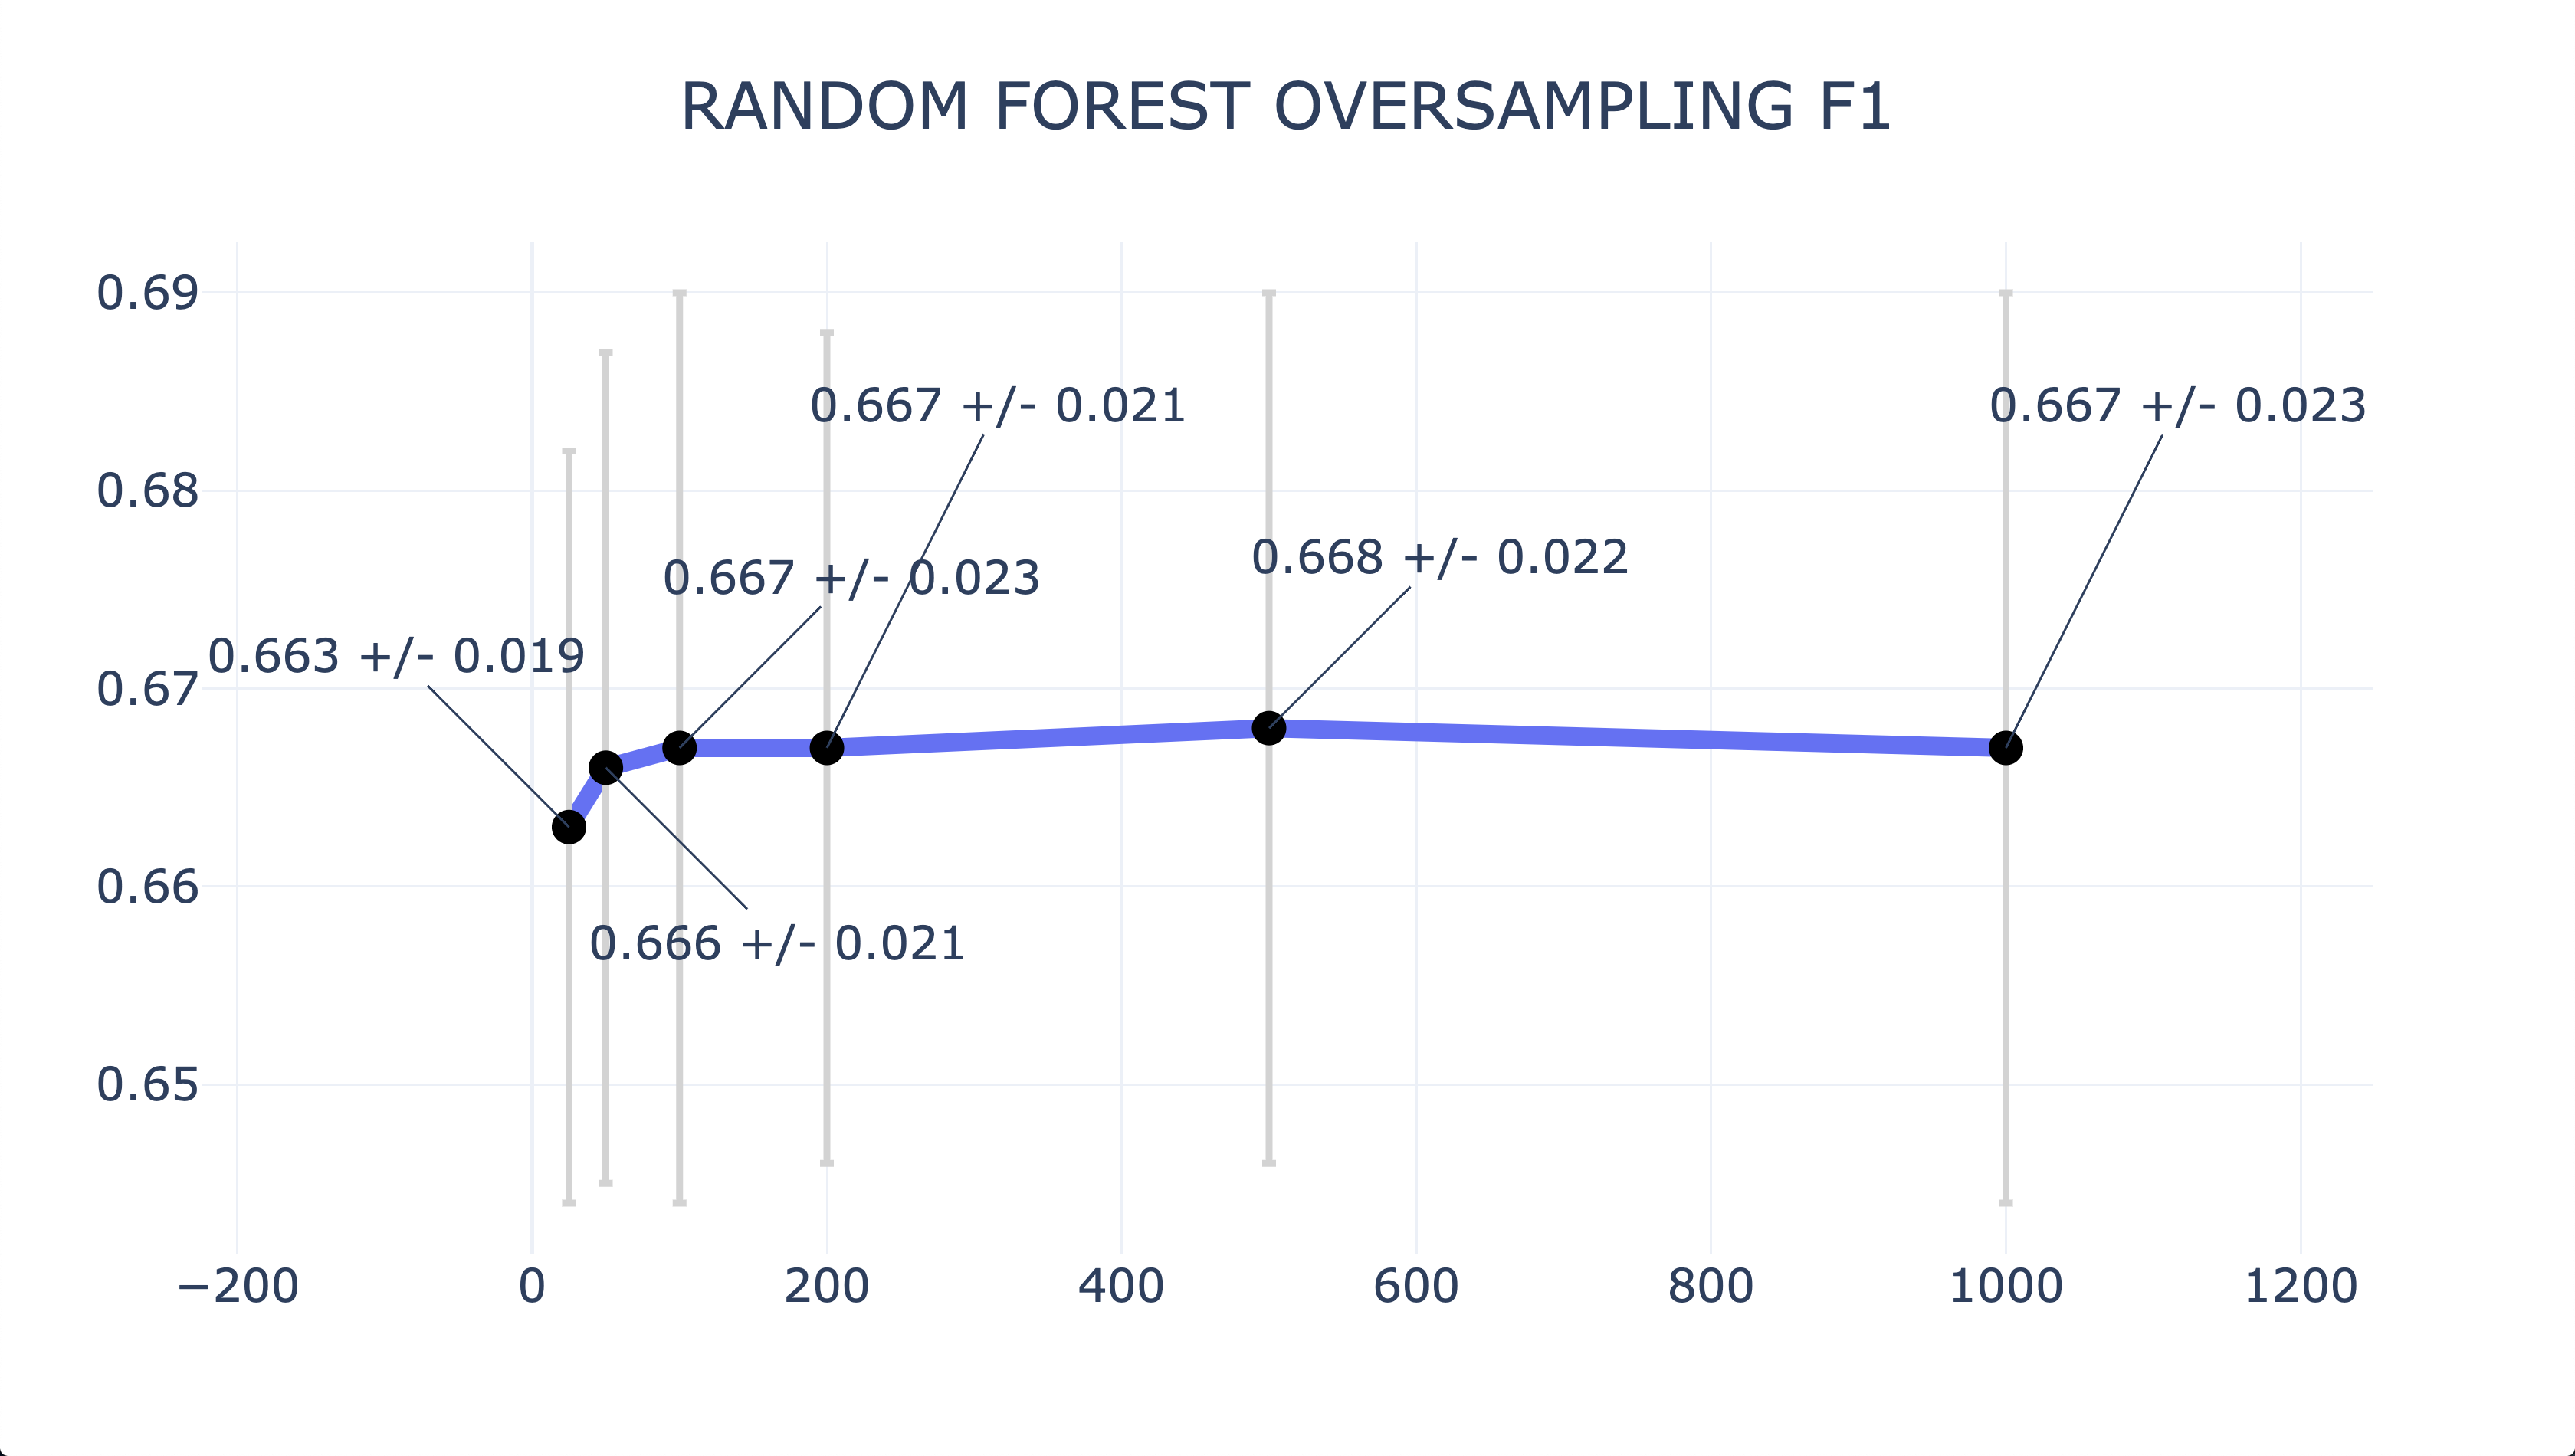
\includegraphics[width=.45\textwidth]{clf_img/RF_OS_f1.png}
		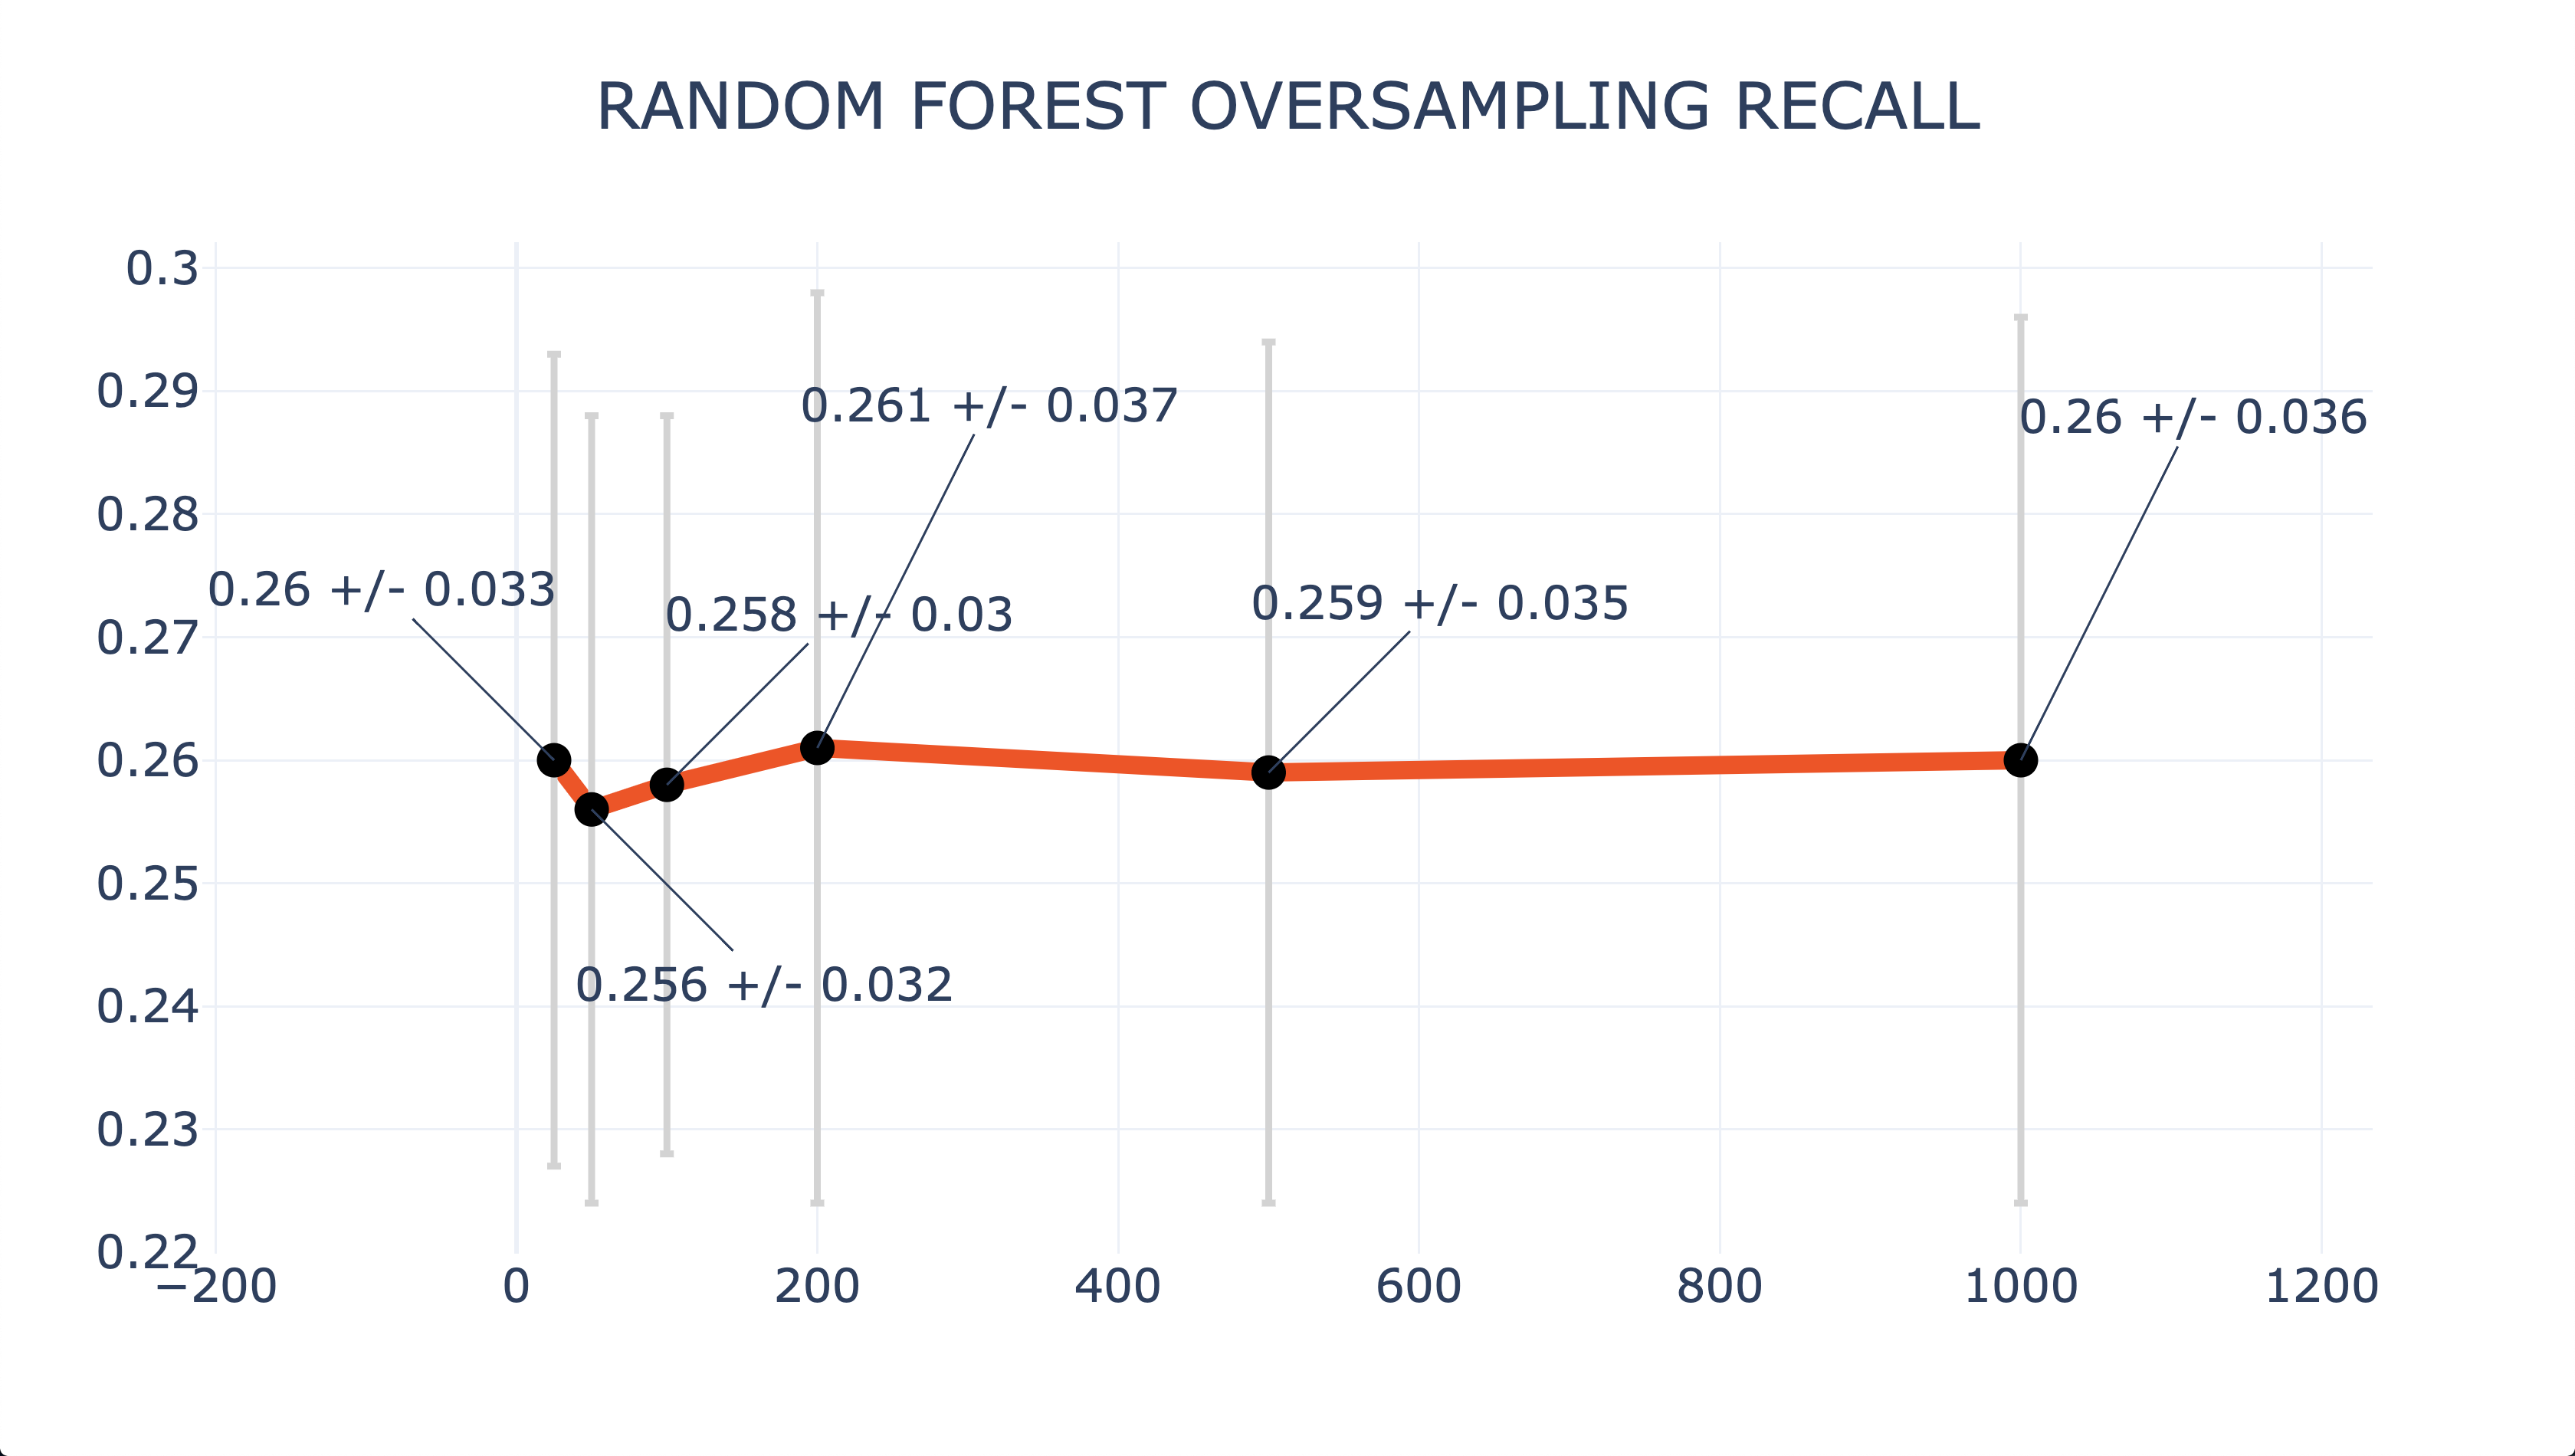
\includegraphics[width=.45\textwidth]{clf_img/RF_OS_recall.png}
	\end{figure}
	\begin{figure}[H]
		\centering
		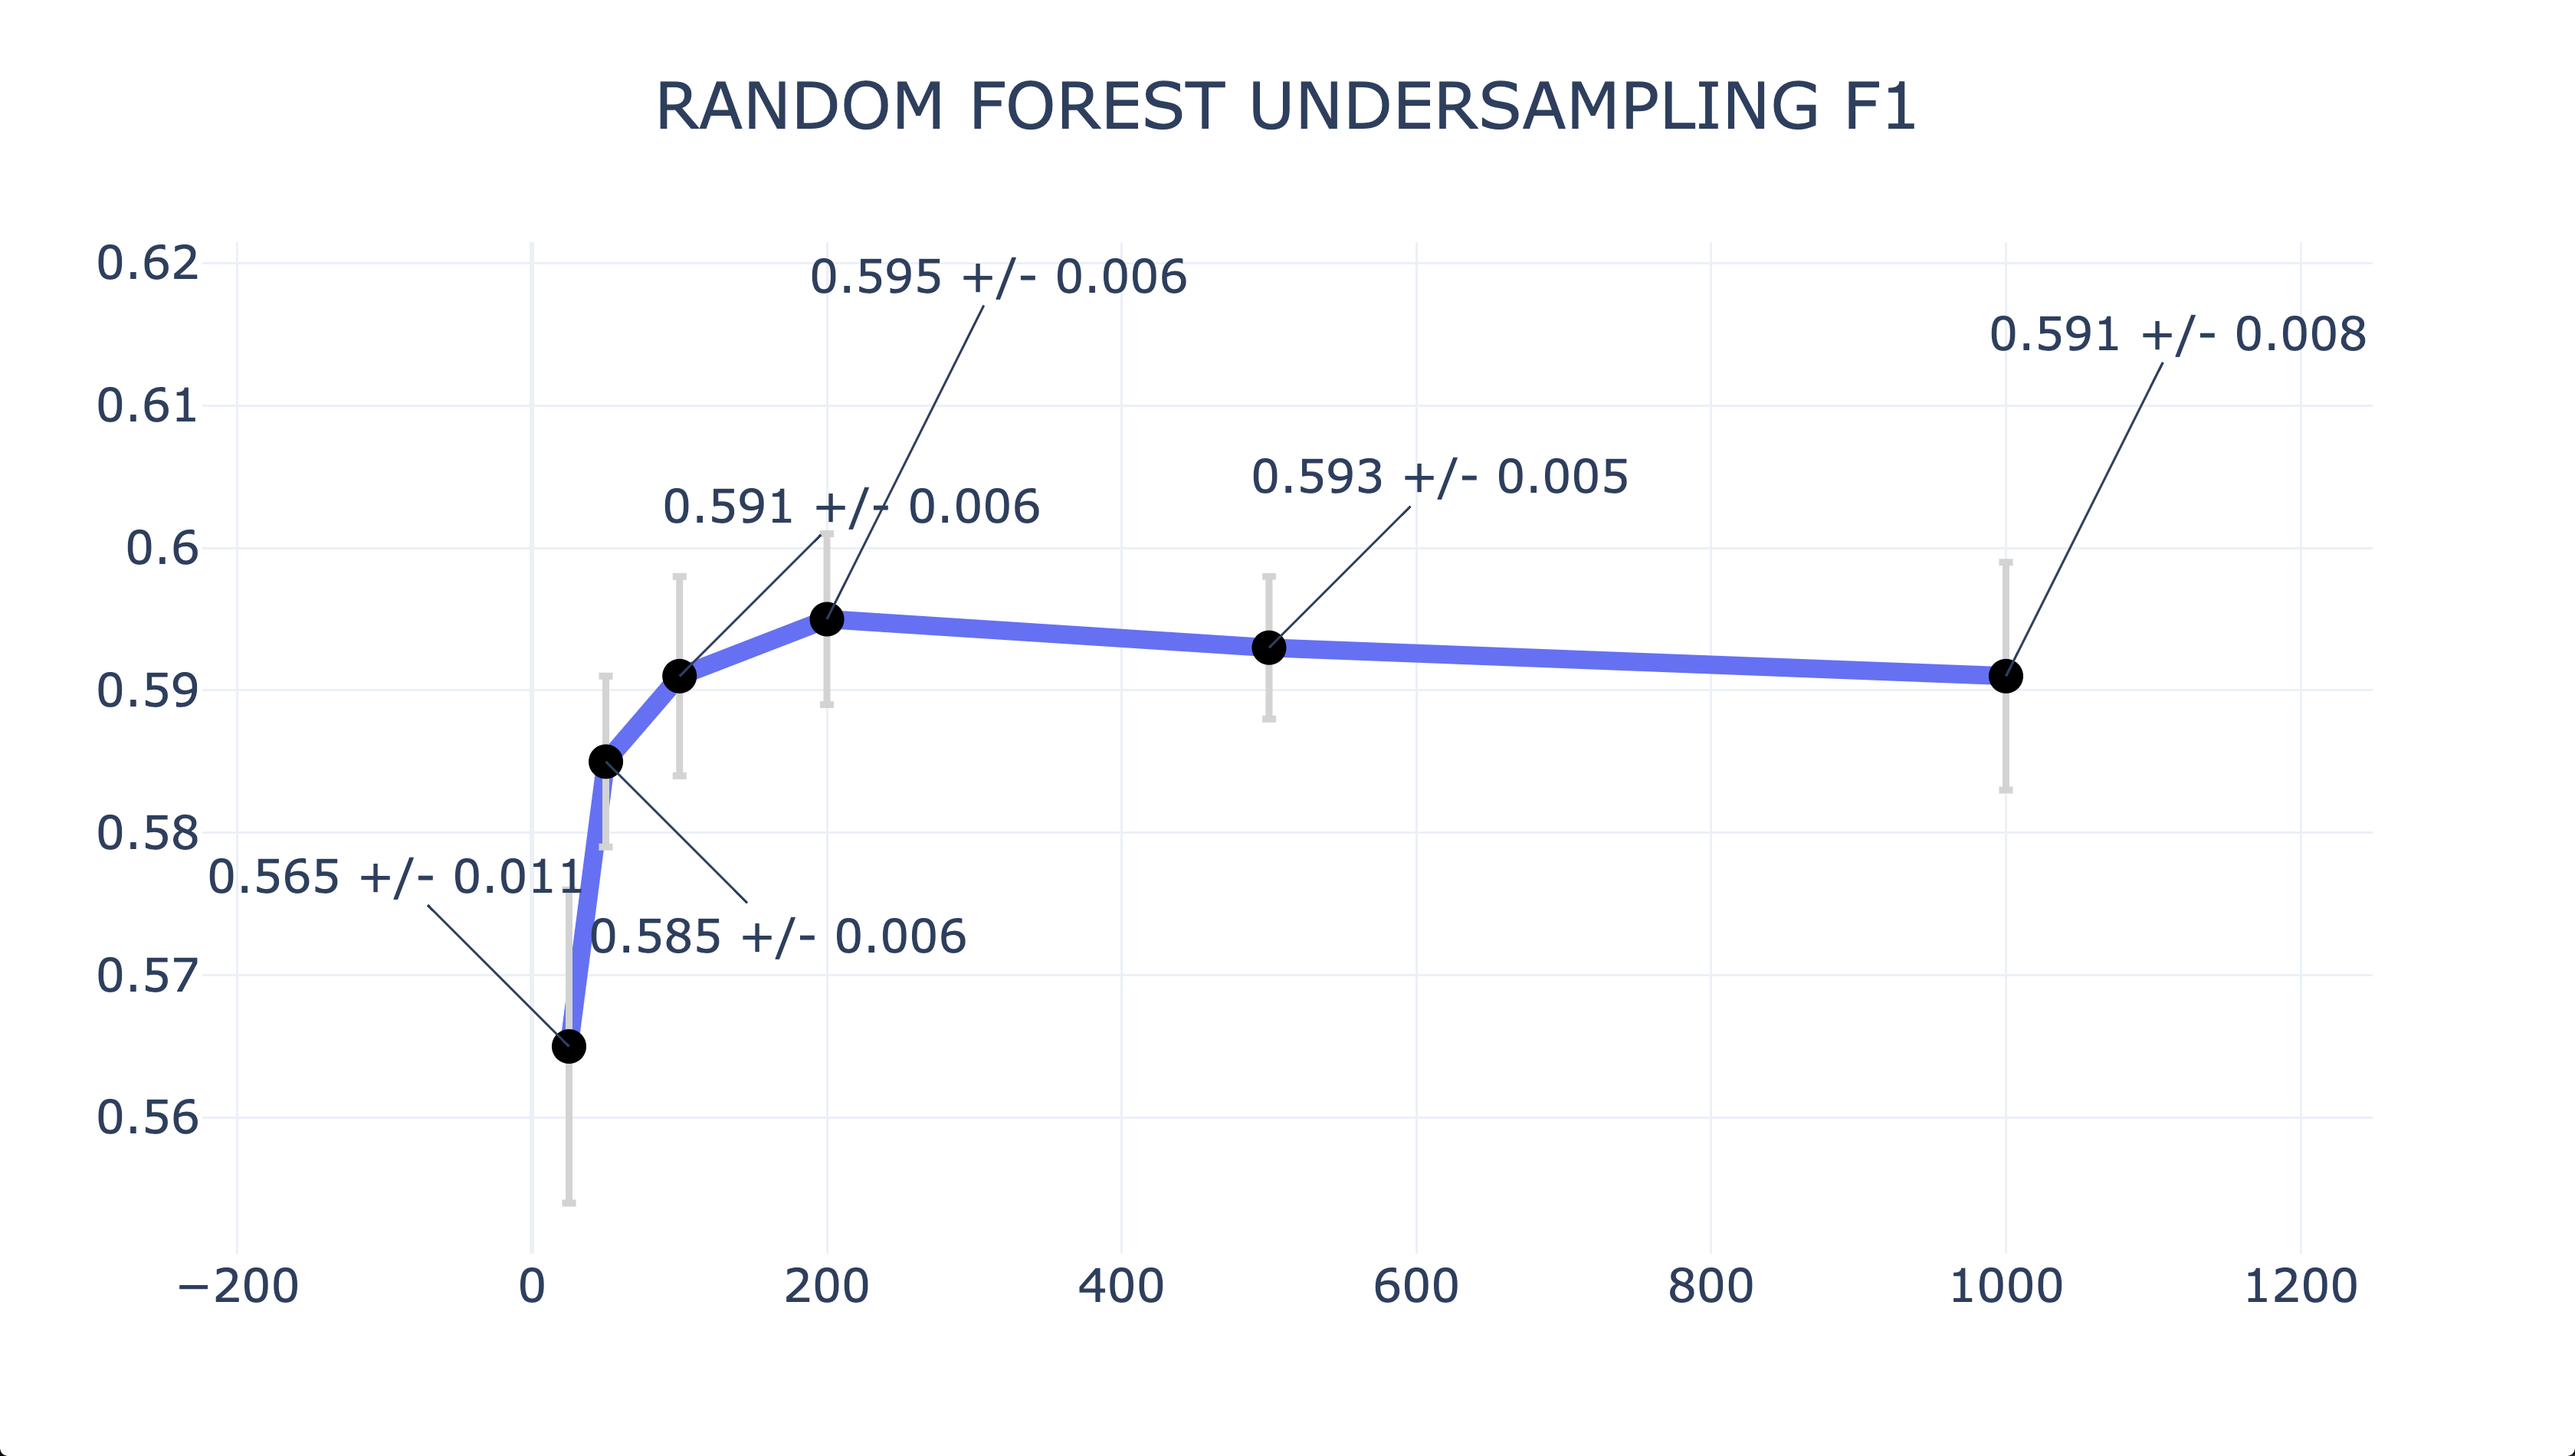
\includegraphics[width=.45\textwidth]{clf_img/RF_US_f1.png}
		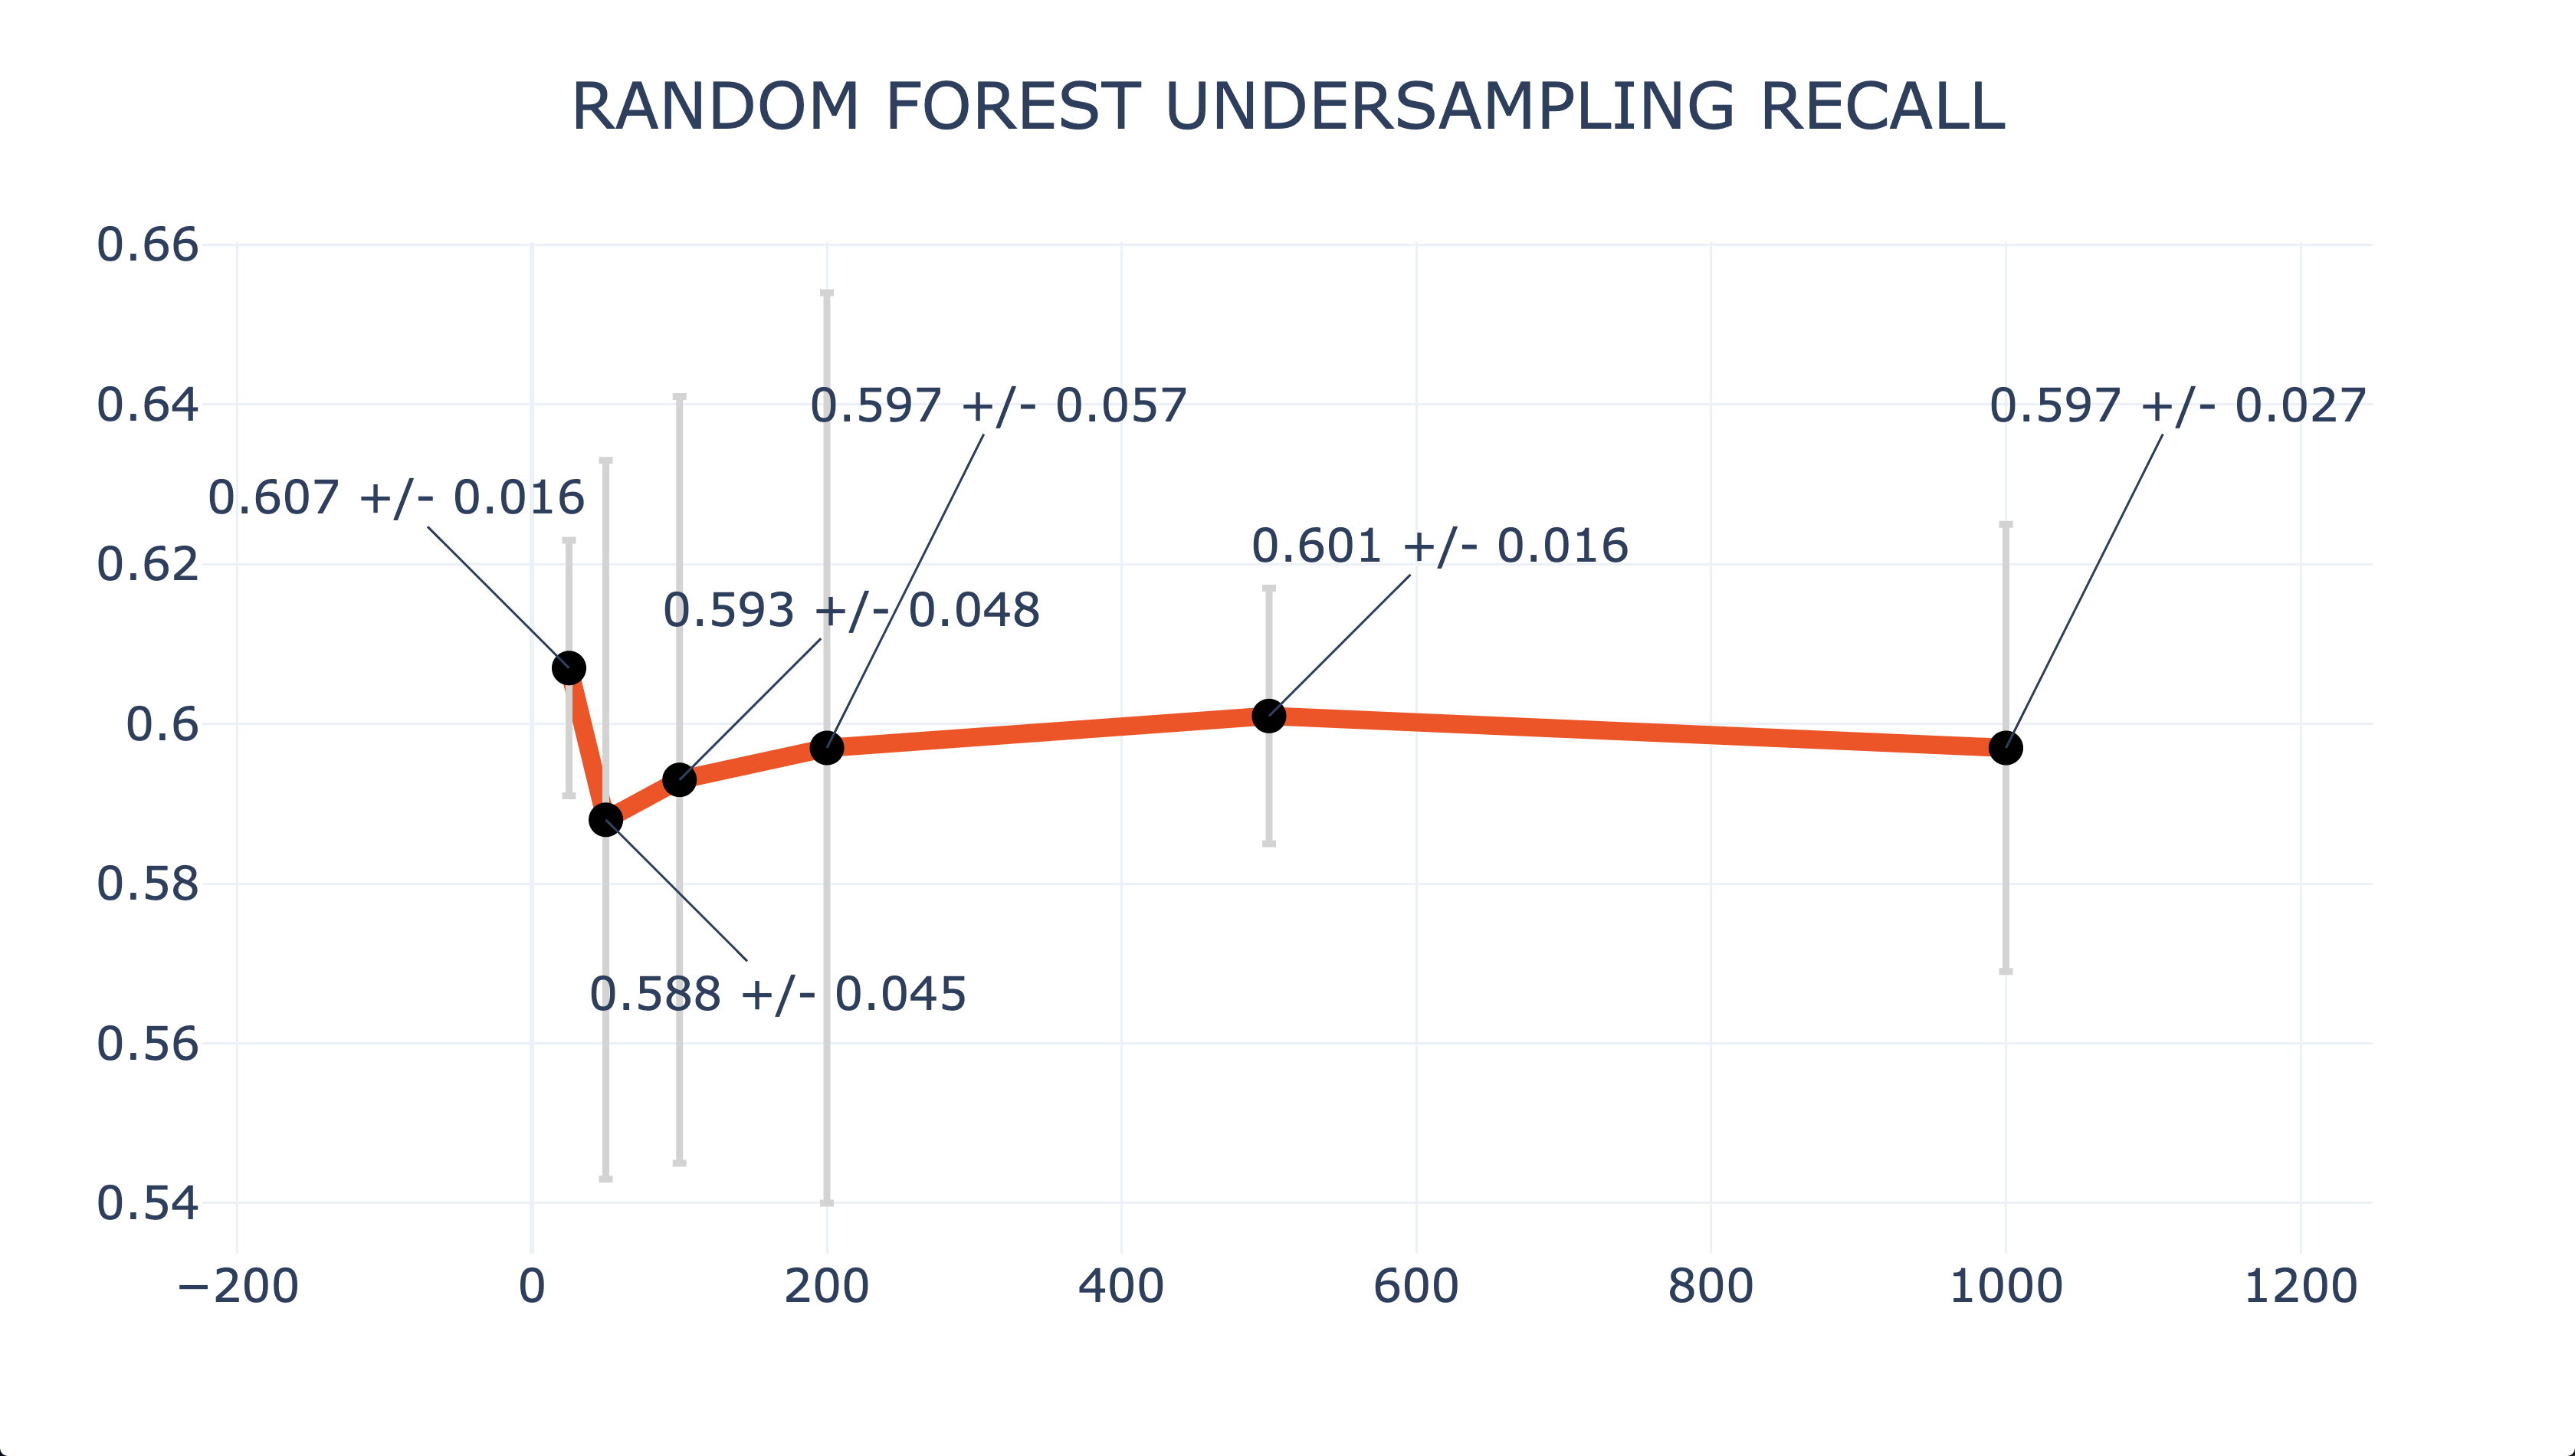
\includegraphics[width=.45\textwidth]{clf_img/RF_US_recall.png}
		\caption{Random Forest tuning}
		\label{fig:hyper_rf}
	\end{figure}
	
	
	\subsubsection{Decision Tree}
	\begin{figure}[H]
		\centering
		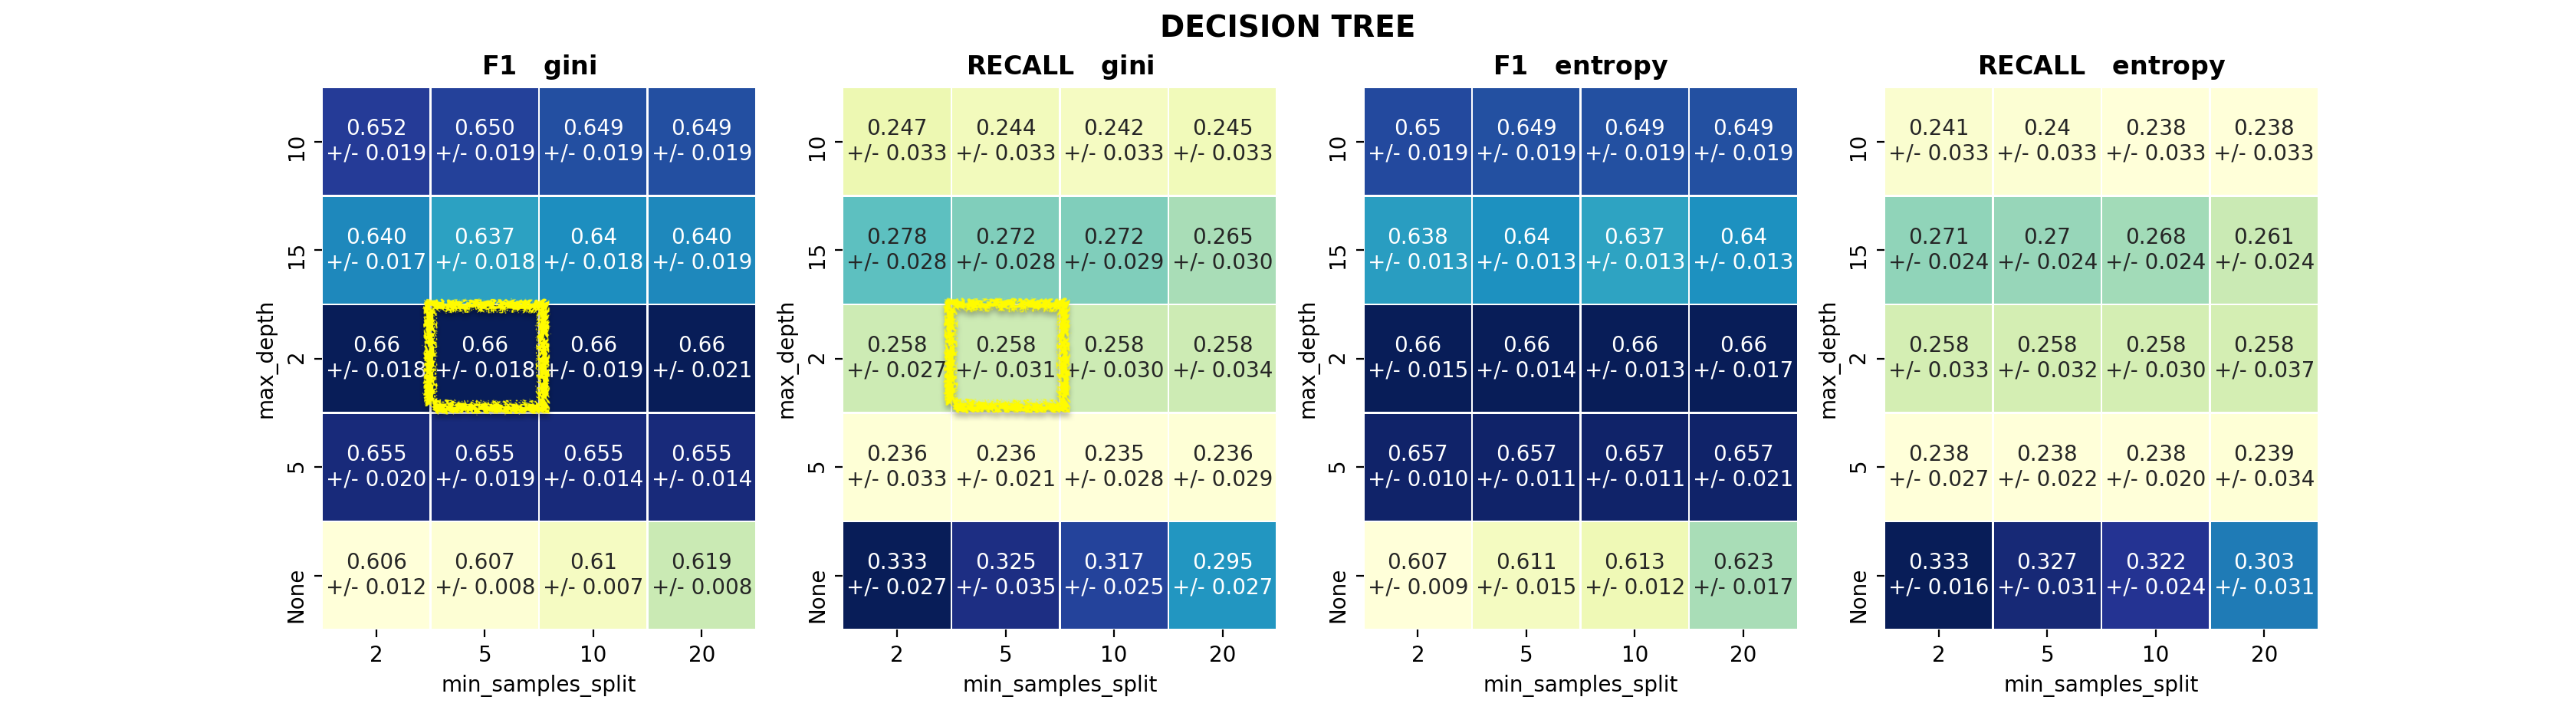
\includegraphics[width=\textwidth]{clf_img/DecisionTree.png}
	\end{figure}
	\begin{figure}[H]
		\centering
		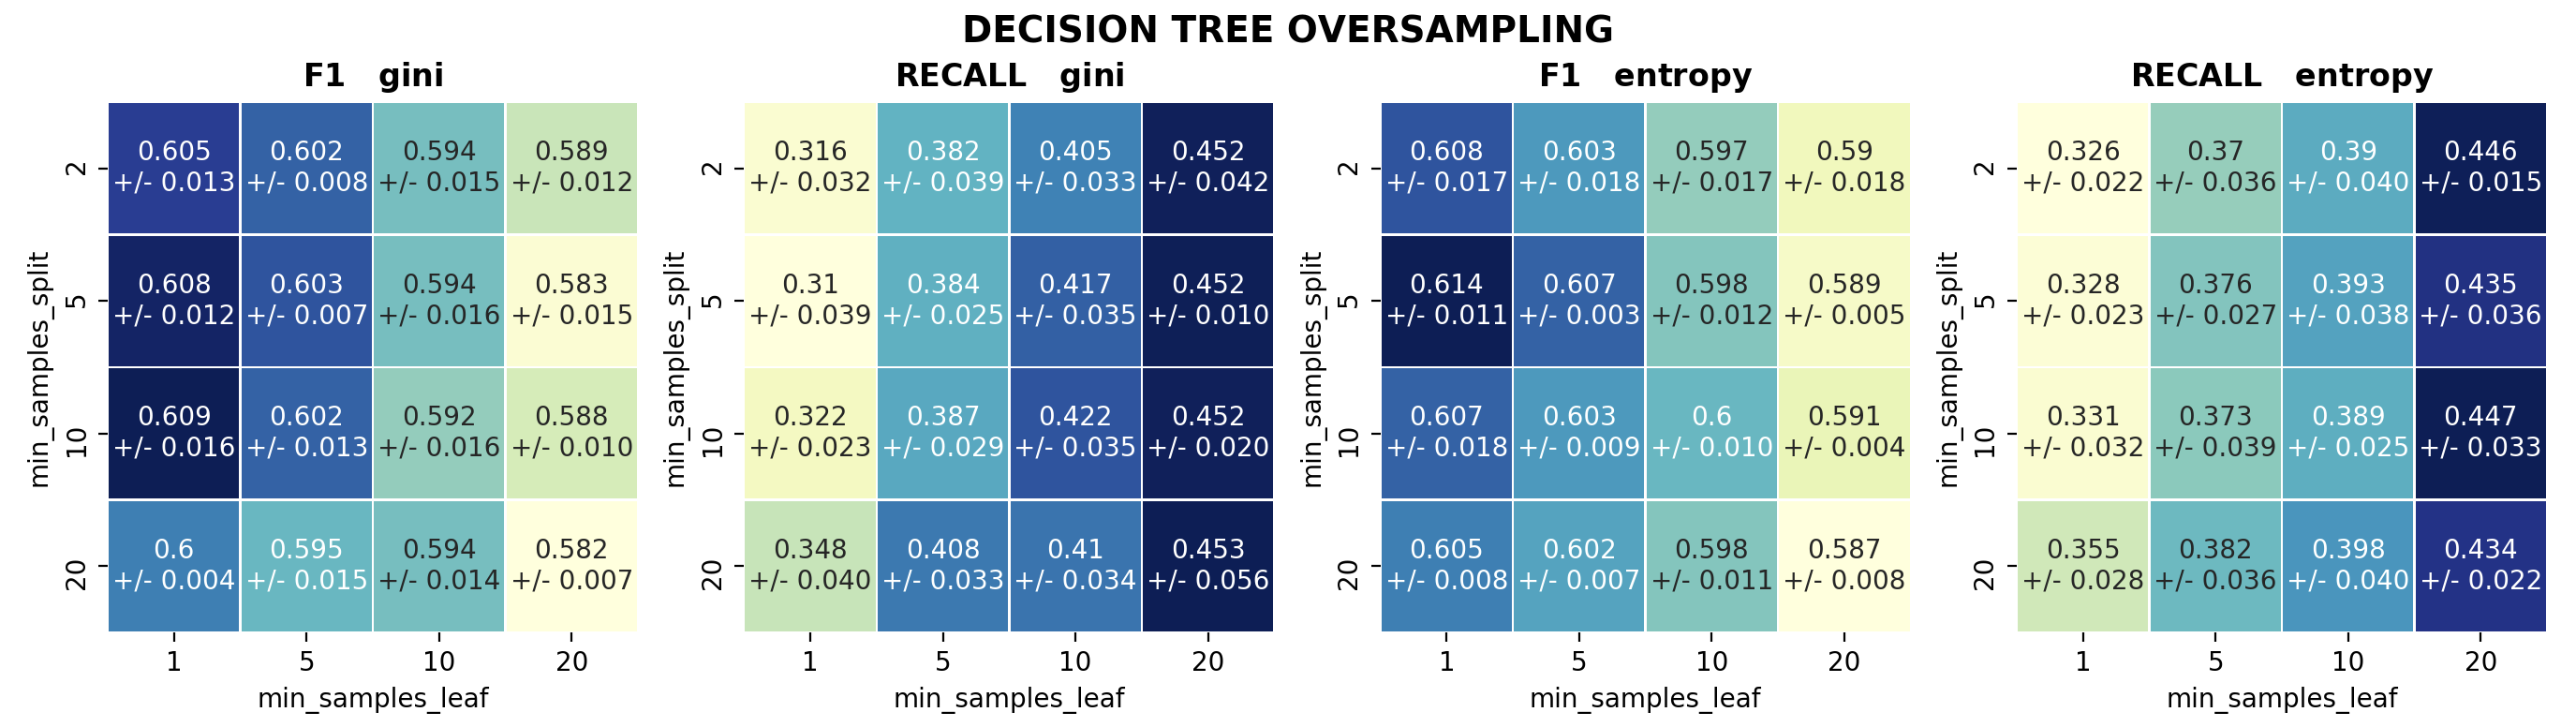
\includegraphics[width=\textwidth]{clf_img/DecisionTree_OS.png}
	\end{figure}
	\begin{figure}[H]
		\centering
		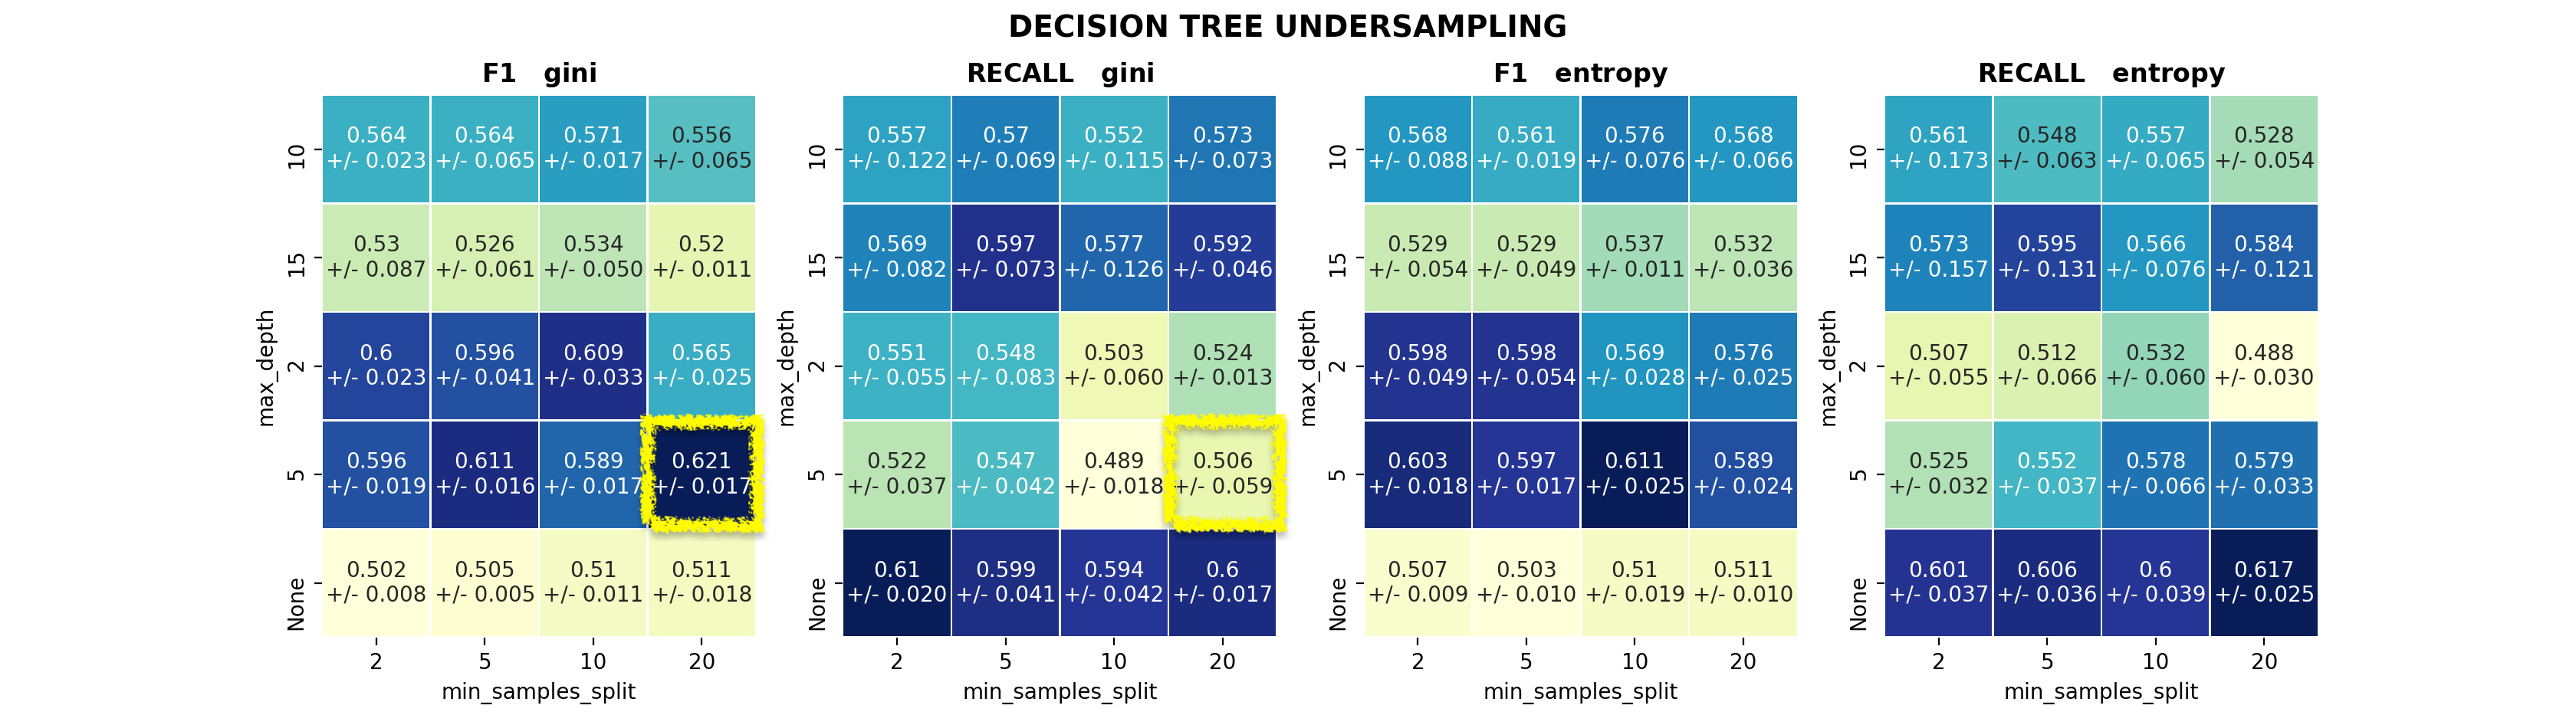
\includegraphics[width=\textwidth]{clf_img/DecisionTree_US.png}
		\caption{Decision Tree tuning}
		\label{fig:hyper_dectree}
	\end{figure}
	
	\subsubsection{AdaBoost}
	\begin{figure}[H]
		\centering
		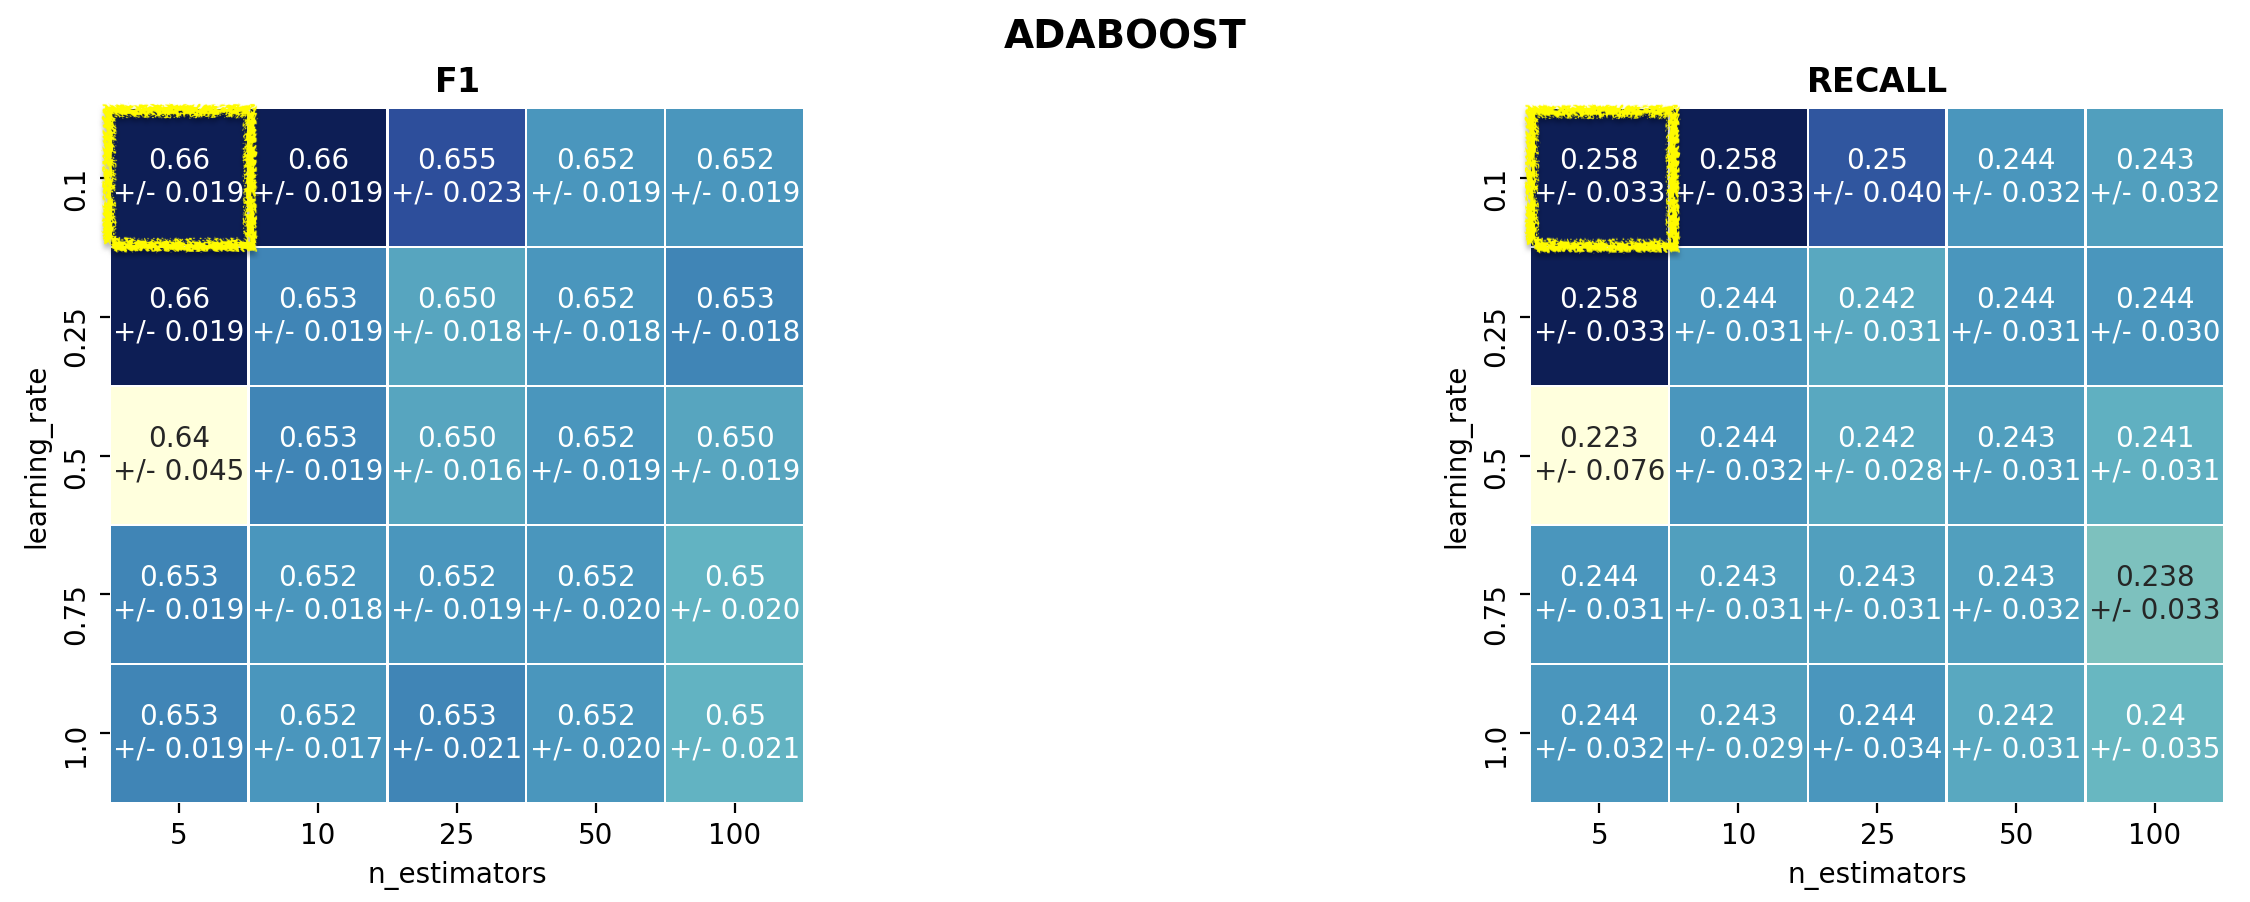
\includegraphics[width=.7\textwidth]{clf_img/Adaboost.png}
	\end{figure}
	\begin{figure}[H]
		\centering
		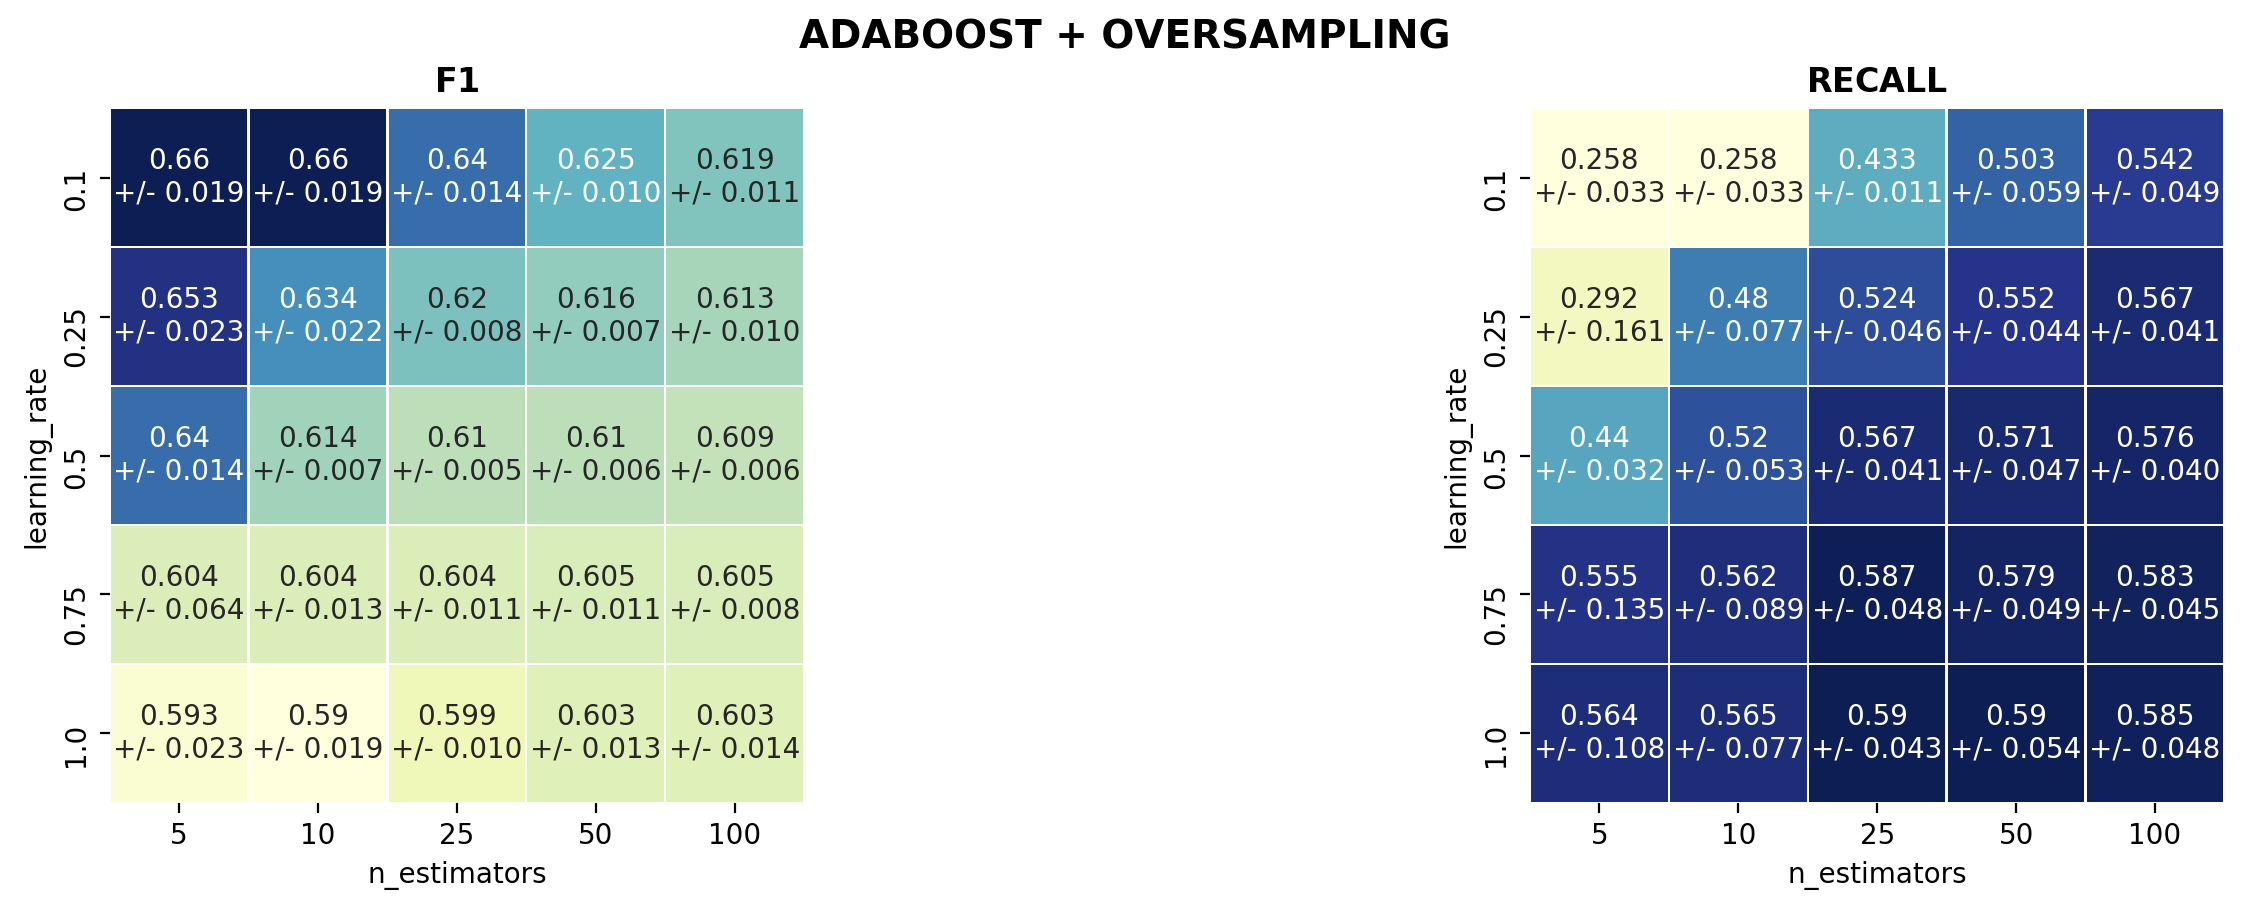
\includegraphics[width=.7\textwidth]{clf_img/Adaboost_OS.png}
	\end{figure}
	\begin{figure}[H]
		\centering
		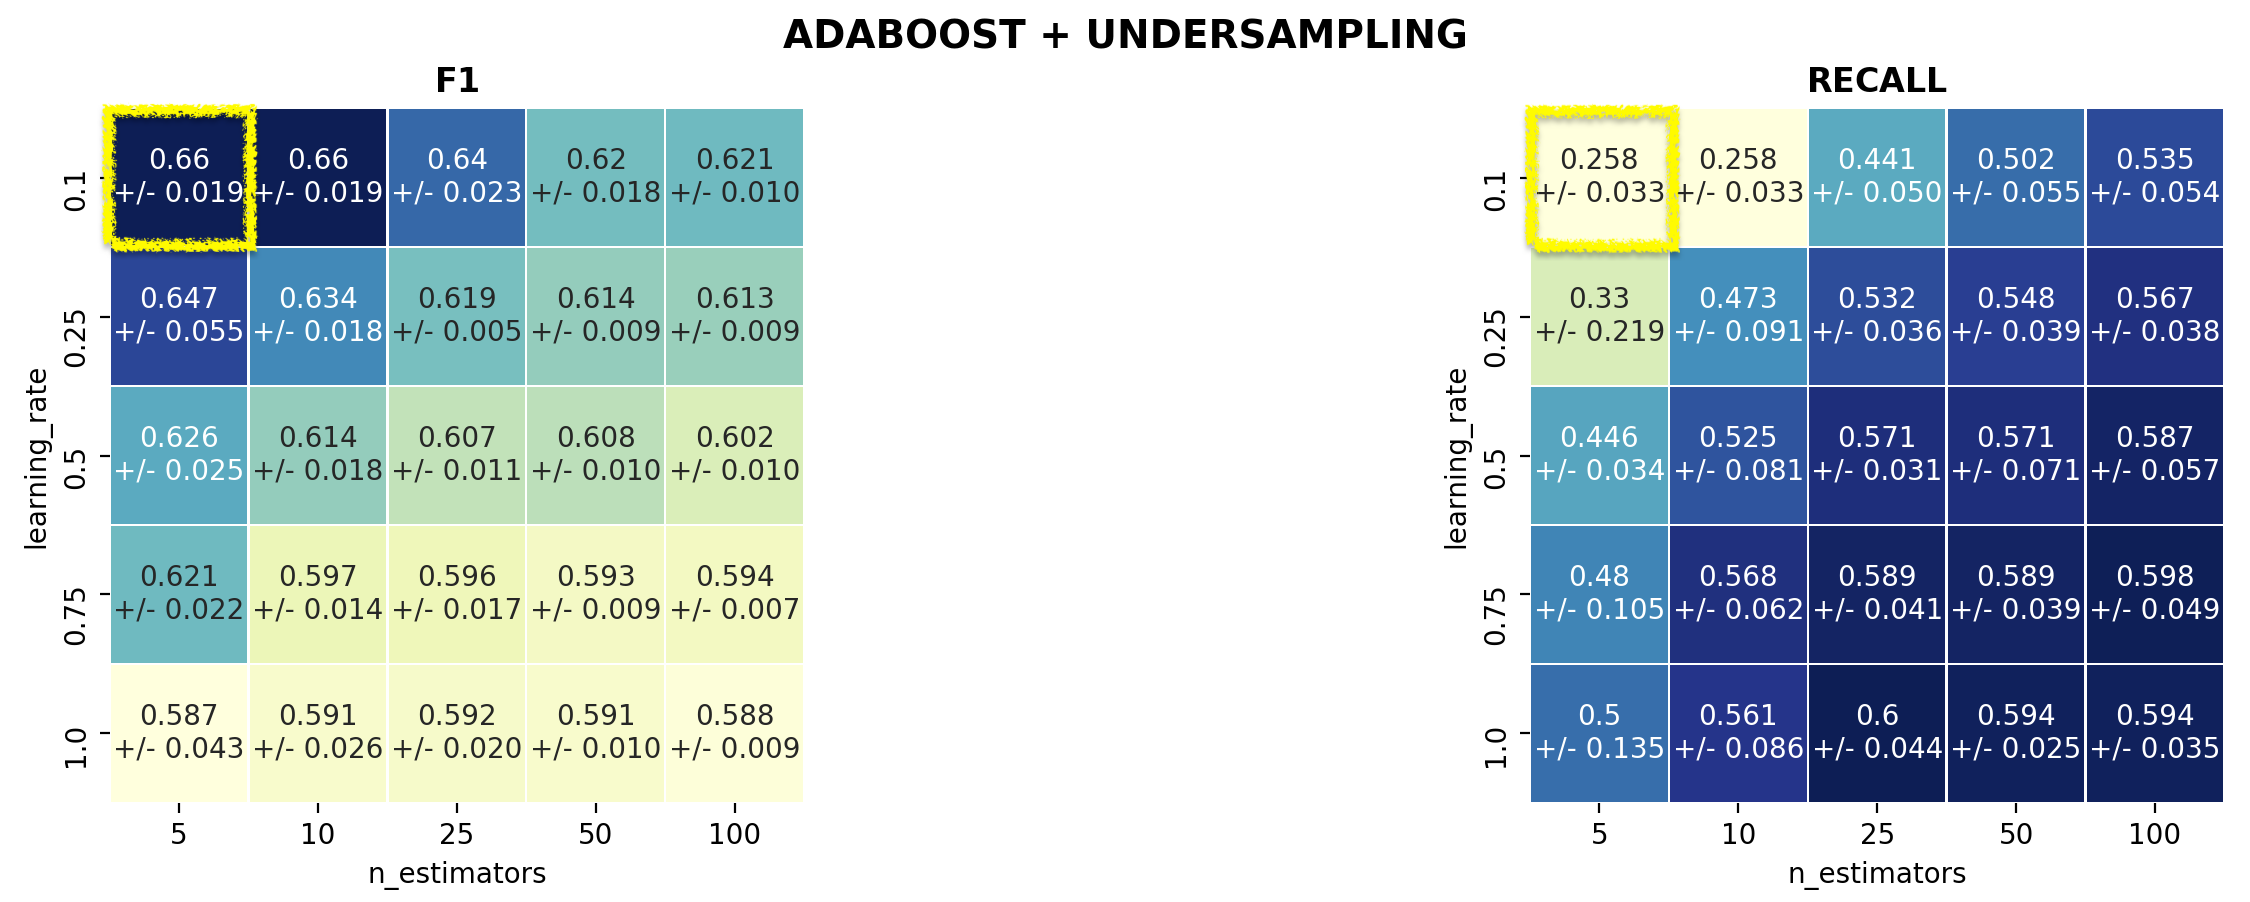
\includegraphics[width=.7\textwidth]{clf_img/Adaboost_US.png}
		\caption{AdaBoost tuning}
		\label{fig:hyper_ada}
	\end{figure}
	
	
	\subsection{Optimized Algorithms : Results}
	Once discovered the best settings for each algorithm, we trained those algorithms using their best parameters. As far as the input data concerns, we adopted the whole training set. Afterwards, we verified the performance using the given test set. Table \ref{tab:restest} highlights that the best approach for this task is Random Forest without any class balancing. 
	
	% Please add the following required packages to your document preamble:
	% \usepackage{multirow}
	% \usepackage[table,xcdraw]{xcolor}
	% If you use beamer only pass "xcolor=table" option, i.e. \documentclass[xcolor=table]{beamer}
	\begin{table}[H]
		\begin{tabular}{c|c|c|c|c|c|c|c|c|c|c|}
			\cline{2-11}
			& \cellcolor[HTML]{656565}{\color[HTML]{FFFFFF} }                                    & \multicolumn{3}{c|}{\cellcolor[HTML]{656565}{\color[HTML]{FFFFFF} \textbf{Precision}}}                                                                            & \multicolumn{3}{c|}{\cellcolor[HTML]{656565}{\color[HTML]{FFFFFF} \textbf{Recall}}}                                                                               & \multicolumn{3}{c|}{\cellcolor[HTML]{656565}{\color[HTML]{FFFFFF} \textbf{F1-Score}}}                                                                             \\ \cline{3-11} 
			& \multirow{-2}{*}{\cellcolor[HTML]{656565}{\color[HTML]{FFFFFF} \textbf{Accuracy}}} & \cellcolor[HTML]{9B9B9B}{\color[HTML]{FFFFFF} 0} & \cellcolor[HTML]{9B9B9B}{\color[HTML]{FFFFFF} 1} & \cellcolor[HTML]{9B9B9B}{\color[HTML]{FFFFFF} \textit{AVG}} & \cellcolor[HTML]{9B9B9B}{\color[HTML]{FFFFFF} 0} & \cellcolor[HTML]{9B9B9B}{\color[HTML]{FFFFFF} 1} & \cellcolor[HTML]{9B9B9B}{\color[HTML]{FFFFFF} \textit{AVG}} & \cellcolor[HTML]{9B9B9B}{\color[HTML]{FFFFFF} 0} & \cellcolor[HTML]{9B9B9B}{\color[HTML]{FFFFFF} 1} & \cellcolor[HTML]{9B9B9B}{\color[HTML]{FFFFFF} \textit{AVG}} \\ \hline
			\rowcolor[HTML]{9AFF99} 
			\multicolumn{1}{|c|}{\cellcolor[HTML]{9AFF99}Random Forest}                 & \textbf{0.90}                                                                      & 0.90                                             & 0.81                                             & \textbf{0.85}                                               & 0.99                                             & 0.22                                             & \textbf{0.61}                                               & 0.95                                             & 0.35                                             & \textbf{0.65}                                               \\ \hline
			\rowcolor[HTML]{E6E6E6} 
			\multicolumn{1}{|c|}{\cellcolor[HTML]{E6E6E6}Random Forest + OverSampling}  & \textbf{0.90}                                                                      & 0.90                                             & 0.78                                             & \textbf{0.84}                                               & 0.99                                             & 0.22                                             & \textbf{0.61}                                               & 0.94                                             & 0.35                                             & \textbf{0.65}                                               \\ \hline
			\multicolumn{1}{|c|}{Random Forest + UnderSampling}                         & \textbf{0.74}                                                                      & \cellcolor[HTML]{FFFFFF}0.92                     & 0.24                                             & \textbf{0.58}                                               & 0.76                                             & 0.54                                             & \textbf{0.65}                                               & 0.84                                             & 0.33                                             & \textbf{0.58}                                               \\ \hline
			\rowcolor[HTML]{E6E6E6} 
			\multicolumn{1}{|c|}{\cellcolor[HTML]{E6E6E6}Decision Tree}                 & \textbf{0.90}                                                                      & 0.90                                             & 0.85                                             & \textbf{0.87}                                               & 0.99                                             & 0.21                                             & \textbf{0.60}                                               & 0.95                                            & 0.34                                             & \textbf{0.64}                                               \\ \hline
			\multicolumn{1}{|c|}{Decision Tree + OverSampling}                          & \textbf{0.72}                                                                      & \cellcolor[HTML]{FFFFFF}0.92                     & 0.23                                             & \textbf{0.58}                                               & 0.75                                             & 0.54                                             & \textbf{0.64}                                               & 0.83                                             & 0.32                                             & \textbf{0.57}                                               \\ \hline
			\rowcolor[HTML]{E6E6E6} 
			\multicolumn{1}{|c|}{\cellcolor[HTML]{E6E6E6}Decision Tree + UnderSampling} & \textbf{0.66}                                                                      & 0.92                                             & 0.20                                             & \textbf{0.56}                                               & 0.66                                             & 0.60                                             & \textbf{0.63}                                               & 0.77                                             & 0.30                                             & \textbf{0.54}                                               \\ \hline
			\multicolumn{1}{|c|}{AdaBoost}                                              & \textbf{0.89}                                                                      & 0.90                                             & 0.68                                             & \textbf{0.79}                                               & 0.99                                             & 0.23                                             & \textbf{0.61}                                               & 0.94                                             & 0.35                                             & \textbf{0.64}                                               \\ \hline
			\rowcolor[HTML]{E6E6E6} 
			\multicolumn{1}{|c|}{\cellcolor[HTML]{E6E6E6}AdaBoost + OverSampling}       & \textbf{0.89}                                                                      & 0.90                                             & 0.68                                             & \textbf{0.79}                                               & 0.99                                             & 0.23                                             & \textbf{0.61}                                               & 0.94                                             & 0.35                                             & \textbf{0.64}                                               \\ \hline
			\multicolumn{1}{|c|}{AdaBoost + OverSampling}                               & \textbf{0.89}                                                                      & 0.90                                             & 0.68                                             & \textbf{0.79}                                               & 0.99                                             & 0.23                                             & \textbf{0.61}                                               & 0.94                                             & 0.35                                             & \textbf{0.64}                                               \\ \hline
		\end{tabular}
		\caption{Results of the optimized algorithm over the test set}
		\label{tab:restest}
	\end{table}
	
	
	
	\subsection{Optimized Decision Tree: Interpretation}
	Although the decision tree is not the best method to predict the required variable, its scores are still valid.
	\begin{wrapfigure}{r}{0.4\textwidth}
		\centering
		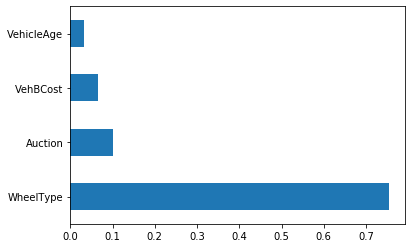
\includegraphics[width=.4\textwidth]{dectreevar.png}
		\caption{Optimized Decision Tree Features Importance}
		\label{fig:optdectreefeat}
	\end{wrapfigure}
	Note that the following pictures refer to the optimized decision tree that has been trained using a max\_depth equal to five (here we're showing only four levels due to lack of space).
	
	Surprisingly enough, the \emph{WheelType} column owns importance that is more than 70\%. Hence, a row having the \emph{WheelType} attribute equal to "NULL" (greater than 3.5) is a potentially risky affair. The second leading variable is the type of auction. In particular, cars sold through "ADESA" (smaller than 1.5) auctions point entirely towards "Bad Buy" leaves. Furthermore, the Gini coefficient (0.412) suggests that this split is almost useless because the preponderant feature is still the previous one. As far as the red branch concerned, there is just one blue leaf. This latter represents the category of cars with a final price above 12260\$ and age less than 4.5.
	
	
	
	
	\begin{figure}[]
		\centering
		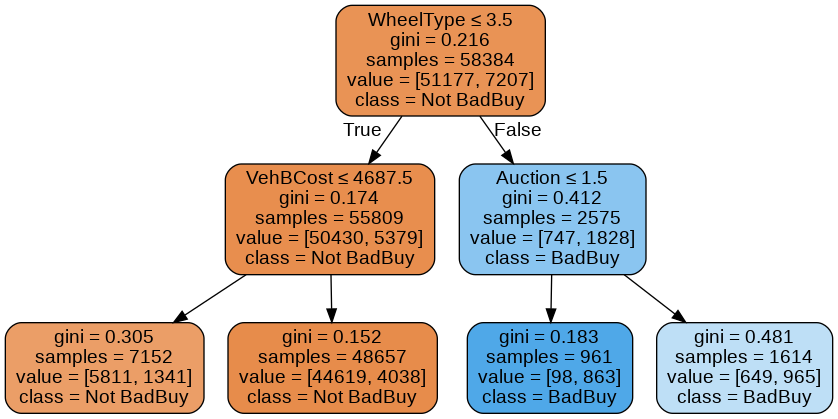
\includegraphics[height=.95\textheight]{dectree.png}
		\caption{Optimized Decision Tree Schema}
		\label{fig:optdectree}
	\end{figure}
	
	\subsection{Optimized Random Forest: Interpretation}
	AAAAA
	
	
	AAAAA
	
	\begin{wrapfigure}{r}{0.4\textwidth}
		\centering
		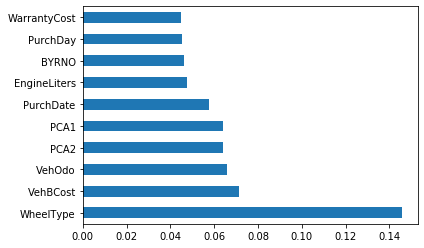
\includegraphics[width=.4\textwidth]{rfw.png}
		\caption{Optimized Random Forest Features Importance}
		\label{fig:optdectree}
	\end{wrapfigure}
	
	AAAAA
	
	
	AAAAA
	
	
	AAAAA
	
	
	\newpage
	\section{Pattern Mining}
	\label{sec:patternmining}
	In this section we try to find the best pattern and association rules in order to better understand the information hidden in the dataset.
	
	\subsection{Attribute selection and binning}
	
	At first, we selected the most informative attributes which are: \emph{VehicleAge, Make, Model, Trim, Color, WheelType, VehOdo, AAAP, BYRNO, VNST, VehBCost, WarrantyCost}.\\
	We chose to use these attributes because most of them are coherent with the data used in the previous analysis.\\  
	To perform this task, we discretized the numerical attributes \emph{VehOdo, VehBCost, WarrantyCost, AAAP, VehicleAge}.\\
	Formerly, we plotted their distribution, and, following the distribution, we chose to split the attributes into five ranges.\\  
	
	\begin{figure}[H]
		\centering
		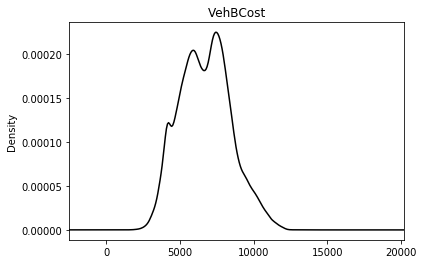
\includegraphics[width=.4\textwidth]{vehbcost}\hspace{1cm}
		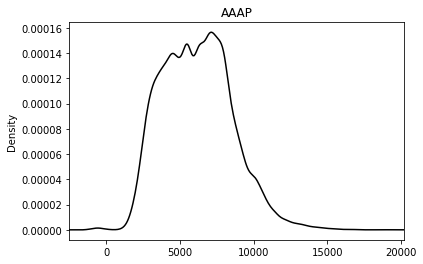
\includegraphics[width=.4\textwidth]{AAAP}
		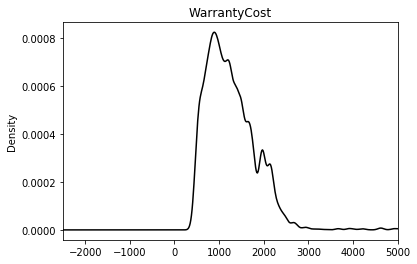
\includegraphics[width=.4\textwidth]{warrantycost}\hspace{1cm}
		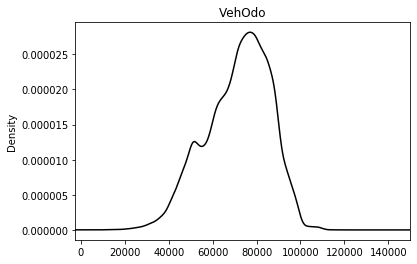
\includegraphics[width=.4\textwidth]{vehodo}
		\caption{Distribution of numerical attributes}
		\label{fig:hyper_rf}
	\end{figure}
	
	In the Figure \ref{fig:hyper_rf}, starting from the left side, we have the distribution of the attribute \emph{VehBCost} on the top (1,5000, 7000, 8000, 10000), and the distribution of \emph{WarrantyCost} on the bottom (1,700, 1200, 1800, 2600). 
	To the right side, the Figure shows the distribution of \emph{AAAP} on the top (1, 3000, 6000, 8000, 10000) and lastly, the attribute \emph{VehOdo} on the bottom (1,40000, 60000, 80000, 100000). 
	
	\subsection{Frequent itemsets extraction}
	
	We ran the Apriori algorithm for frequent itemsets extraction based on the attributes that produced the best results in the previous analysis. Furthermore, we decided to drop some attributes like \emph{Transmission, Nationality} and \emph{SubModel}, because they produced patterns which were too generic and, as a consequence, the results were not meaningful. This behaviour depends on the strong imbalance between the two classes.\\
	Subsequently, we try to extract frequent patterns with different values of support by using frequent, maximal and closed types.\\
	After several attempts, we agreed that the best min\_support was between 9\% and 11\%, selecting only sets that have three elements. Nevertheless, probably for the low amount of attributes that we used for this task, even though we used different types (\emph{frequent}, \emph{maximal}, and \emph{closest}) of support, the results produced were the same, which are shown in Table \ref{tab:boh}.\\
	We noticed that the number of patterns changes substantially by increasing support. Indeed, by using support of 2\%  we obtained 1467 patterns, a number which is three times lower than the previous one (5759 with support 1\%).\\
	The distribution of patterns is represented in a \emph{logarithmic scale} in Figure \ref{fig:hyper_rf_us}.
	
	
	\begin{figure}[H]
		\centering
		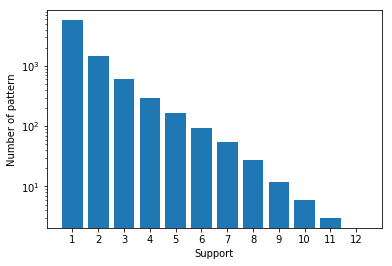
\includegraphics[width=.4\textwidth]{support.png}
		\caption{Frequency plot of itemsets with different support values represented on a \textbf{logarithmic scale}.}
		\label{fig:hyper_rf_us}
	\end{figure}
	
	
	
	\begin{table}[H]
		\centering
		\begin{tabular}{|c|c|}
			\hline
			\textbf{Pattern} & \textbf{Support} \\
			\hline
			\rowcolor{Gray}
			VehBCost:(5000.0, 7000.0], AAAP:(3000.0, 6000.0], Age:[4, 6) &  6798\\
			VehBCost:(5000.0, 7000.0], AAAP:(3000.0, 6000.0], Covers &  6653\\
			\rowcolor{Gray}
			AAAP:(3000.0, 6000.0], Age:[4, 6), Covers &  6458\\
			Age:[4, 6), Odo:(60000, 80000], Alloy &  6392\\
			\rowcolor{Gray}
			AAAP:(3000.0, 6000.0], Age:[4, 6), Odo:(60000, 80000] &  6222\\
			VehBCost:(5000.0, 7000.0], AAAP:(3000.0, 6000.0]', Odo:(60000, 80000]  & 5936\\
			\rowcolor{Gray}
			AAAP:(3000.0, 6000.0], Age:[4, 6), Alloy &  5794\\
			WarrCost:(1200, 1800], Odo:(60000, 80000], Alloy & 5641\\
			\rowcolor{Gray}
			VehBCost:(5000.0, 7000.0], AAAP:(3000.0, 6000.0], Alloy &  5410\\
			VehBCost:(5000.0, 7000.0], Covers, Odo:(60000, 80000] & 5373\\
			\rowcolor{Gray}
			AAAP:(3000.0, 6000.0], Age:[4, 6), Alloy & 5794\\
			WarrCost:(1200, 1800], Odo:(60000, 80000], Alloy & 5641\\
			\rowcolor{Gray}
			VehBCost:(5000.0, 7000.0], AAAP:(3000.0, 6000.0], Alloy & 5410\\
			VehBCost:(5000.0, 7000.0], Covers, Odo:(60000, 80000] & 5373\\
			\rowcolor{Gray}
			AAAP:(3000.0, 6000.0], Odo:(60000, 80000], Alloy & 5306\\
			WarrCost:(700, 1200], Odo:(60000, 80000], Alloy & 5266\\\hline
		\end{tabular}
		\caption{Pattern of different types with support between 9\% and 11\%}
		\label{tab:boh}
	\end{table}
	
	From the generated itemsets we can see that cars which are not new but neither old, are usually sold at a slightly more expensive price compared to the average price at the auction (Pattern 1 in the Table, which is the one with highest frequency). The mileage on the vehicle is usually between 60000 and 80000 (Pattern 5) for cars that have an average price between 3000.0 and 6000.0 and age between 4 and 6.\\ %rivedere questa frase
	The attributes in these patterns are very meaningful since they are the same that give us the best results in clustering analysis section. 
	
	
	\subsection{Association Rules}
	In this section, we discuss the most interesting association rules obtained with the Apriori algorithm. 
	We decided to attempt extracting these rules considering support up to 100\%, length of maximum three elements and confidence lower or equal than 70\%. We show in Figure \ref{fig:hyper_rf} how the number of rules varies by varying the confidence value (confidence is between 65\% and 67\% in the plot). We also plotted, on the right, a scatter plot showing confidence, support and lift. We can notice that the number of rules with $\mathbf{support} >= 10$ is very low with respect to the whole amount.
	
	
	\begin{figure}[]
		\centering
		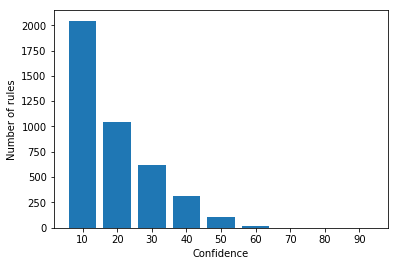
\includegraphics[width=.4\textwidth]{rules.png}\hspace{1cm}
		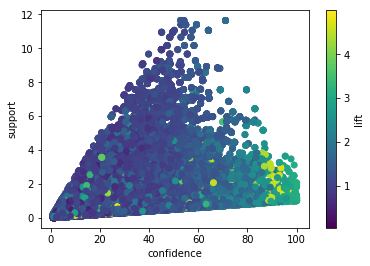
\includegraphics[width=.4\textwidth]{AbusivismoEdilizio.png}
		\caption{On the lefthand side, frequency plot of rules by varying the confidence value. On the righthand side, a scatter plot of support, lift and confidence}
		\label{fig:hyper_rf}
	\end{figure}
	
	We found optimal results with $\mathbf{support} = 11$ and $\mathbf{confidence} \approx 67\%$.  
	The association rules found with those optimal parameters are shown in Table 7.
	
	\begin{table}[H]
		\centering
		\begin{tabular}{|cc|cc|}
			\hline
			\textbf{RHS} & \textbf{LHS} & \textbf{Confidence} & \textbf{Lift} \\
			\hline
			\rowcolor{Gray}
			GM & LS & 0.768 & 2.273\\
			GM & WarrCost:(1800, 2600] & 0.736 & 2.177\\
			\rowcolor{Gray}
			CHRYSLER & Odo:(40000, 60000], WarrCost:(700, 1200] & 0.689 & 2.149\\
			Alloy & FORD  & 0.767 & 1.523\\
			\rowcolor{Gray}
			Covers & Age:[2, 4), VehBCost:(5000.0, 7000.0]  & 0.687 & 1.501 \\
			Alloy &  Odo:(80000, 100000], WarrCost:(1200, 1800] &  0.678 & 1.346 \\
			\hline
		\end{tabular}
		\caption{Most significant association rules with optimal parameters}
		\label{tab:rules}
	\end{table}
	
	As we can see from Table \ref{tab:rules}, General Motors vehicles (GM) are usually LS series, with the highest confidence and lift. Among the American car makes, Chrysler is the one that has the lowest average warranty cost as we can also see in Figure \ref{fig:fantastic}. 
	
	
	\subsubsection{Association Rules for missing value replacement}
	
	After performing data Preparation for pattern mining, we decided to attempt replacing the missing value of the attribute \emph{WheelType}, the only one which contains missing values.\\
	For a maximum of three elements, we used $\mathbf{support}= 11$ and we selected as confidence between 0.67\% and 0.76\% to find the best rules.
	Then, we chose the most interesting rules for the most frequent elements within \emph{WheelType}(\emph{Alloy} and \emph{Covers}) and we replaced only the value 'Unknown' by following the rules extracted.  \\
	The rules we chose replaced exactly 935 elements out of a total of 2575 missing values, obtaining coverage of 36,31\%.\\
	
	
	\begin{table}[H]
		\centering
		\begin{tabular}{|cc|cc|}
			\hline
			\textbf{RHS} & \textbf{LHS} & \textbf{Confidence} & \textbf{Lift} \\
			\hline
			\rowcolor{Gray}
			Alloy & FORD  & 0.767 & 1.523\\
			Covers & Age:[2, 4), VehBCost:(5000.0, 7000.0]  & 0.687 & 1.501 \\
			\rowcolor{Gray}
			Alloy &  Odo:(80000, 100000], WarrCost:(1200, 1800] &  0.678 & 1.346 \\
			\hline
		\end{tabular}
		\caption{Most significant association rules for missing value replacement}
		\label{tab:missingvalrules}
	\end{table}
	
	
	\subsubsection{Association Rules for predicting target variable}
	To predict the target variable we decided to perform \emph{undersampling} in order to balance the number of 'BadBuy' and 'GoodBuy' for producing not only association rules for 'GoodBuy', which are the majority of attributes, but also for 'BadBuy'.\\
	We selected the most significant rules by using $\mathbf{support}=10$ and $\mathbf{confidence} = 0.67$ and then, we selected rules with a higher confidence and lift.\\
	We used those rules to predict the target variable, and whenever they did not match any element in the data frame, we decided to predict them as 'GoodBuy', since it represents the majority class. \\
	The result of this process is described in Table \ref{tab:predict}, whereas the confusion matrix is shown in Table \ref{tab:confusion}.
	From this table, we compute the accuracy which is 83\%.
	
	\begin{table}[H]
		\centering
		\begin{tabular}{|cc|cc|}
			\hline
			\textbf{RHS} & \textbf{LHS} & \textbf{Confidence} & \textbf{Lift} \\
			\hline
			\rowcolor{Gray}
			GoodBuy & AAAP:(6000.0, 8000.0], Covers  & 0.701 & 1.402 \\
			GoodBuy & Age:[2, 4), Covers & 0.686 & 1.373 \\
			\rowcolor{Gray}
			GoodBuy &  CHRYSLER, Covers &  0.647 & 1.295 \\
			BadBuy &  VehBCost:(224.0, 5000.0], AAAP:(3000.0, 6000.0] & 0.613 & 1.226\\
			\hline
		\end{tabular}
		\caption{Most significant association rules for prediction the target variable}
		\label{tab:predict}
	\end{table}
	
	\begin{table}[H]
		\centering
		\begin{tabular}{cc|cc}
			\multicolumn{1}{c}{} &\multicolumn{1}{c}{} &\multicolumn{1}{c}{\textbf{Predicted Value}} \\ 
			\multicolumn{1}{c}{} & 
			\multicolumn{1}{c|}{} & 
			\multicolumn{1}{c}{\textbf{Yes}} & 
			\multicolumn{1}{c}{\textbf{No}} \\ \hline
			\multirow{2}{*}{\rotatebox{1}{\textbf{Actual Value}}}
			& \textbf{Yes}  & 47548 & 3629   \\ 
			& \textbf{No}  & 6295  & 912 \\ \hline
		\end{tabular}
		\caption{Confusion matrix obtained from the application of the association rules for the target variable prediction. }
		\label{tab:confusion}
	\end{table}
	\addvspace{0.9cm}
	
	If we compare these results with the ones obtained in the Classification (Section \ref{sec:classification}), we can note that:
	\begin{itemize}
		\item the number of True Positive is similar;
		\item the number of True Negative is lower;
		\item the number of False Positive is almost the same;
		\item the number of False Negative is very high.
	\end{itemize}{}
	
	Since we use only four rules for predicting the target variable, we can evaluate it as a good result.
	
	
	\section{Conclusion}
	
	For the analysis of this car auctions data set, we used different data mining techniques, trying to understand whether a deal is a good transaction or not. \\
	In the \emph{Data Understanding} section, we addressed issues related to data semantics and quality, like fixing missing values and deleting redundant variables. Our main goals were to clean up the \emph{Model} variable (which we believed to be one of the deciding factors for the target variable), to reduce the dimensionality of highly correlated variables and have a basic understanding of variable distributions.\\
	In the \emph{Clustering} section, we concentrated our focus on numeric attributes (prices, odometer and warranty cost) to find groups of similar points in the data set. We found, as an obstacle, the main cluster of points of various densities. We found KMeans and Hierarchical clustering to be the best in performance, and attempted to describe the meaning of given results.\\
	In the \emph{Classification} phase, we tried to predict the value of the target variable, namely \emph{IsBadBuy}. We performed 5-fold cross-validation with various classifiers and configurations, attempting also both \emph{undersampling} and \emph{oversampling}. We optimized the parameters for \emph{F1 score} and obtained $\mathbf{F1}_{avg} = 0.65$ on the test set with the best classifier. The accuracy is very high, but the classifier does not obtain better results because of the recall on the negative class (the minority one).  \\
	Lastly, in the \emph{Pattern Mining} phase, we obtained some interesting rules by discarding highly imbalanced categorical attributes. We were able to obtain decent results both when attempting to predict the target variable and when replacing the missing values.
	
\end{document}


